\documentclass{article}
\usepackage[utf8]{inputenc}
\usepackage{amsmath,amsfonts,amssymb}
\usepackage{graphics}
\usepackage{float}
\usepackage{indentfirst}
\usepackage{mathtools}
\usepackage{subfigure}
\usepackage[pdftex]{hyperref}
\usepackage[pdftex]{color,graphicx}

\title{
\normalfont \normalsize 
\textsc{EMAp - Escola de Matemática Aplicada \\ 
Fundação Getúlio Vargas} \\
[10pt] 
\rule{\linewidth}{1pt} \\[6pt] 
\huge Relatório Linguagens de Programação \\
\rule{\linewidth}{1pt}  \\[6pt]
}
\author{Breno Russo Guedes, Cientista de Dados\\
Ademir Tomaz, Engenheiro de Dados\\
Luiz Antônio Granja, Engenheiro de Dados\\
Tulio Koneçny, Especialista em Visualização de Dados\\
Luigi Mezzogori, Especialista de Garantia da Qualidade\\}
\date{\normalsize {Dezembro, 2020}}

\begin{document}

\maketitle

\section{UFC}
\subsection{Resultado de Análises}
\textbf{1.} Como ocorre a distribuição por gênero? Existe uma categoria que mulheres estão mais presentes que os homens?

\begin{figure}[H]
    \centering
    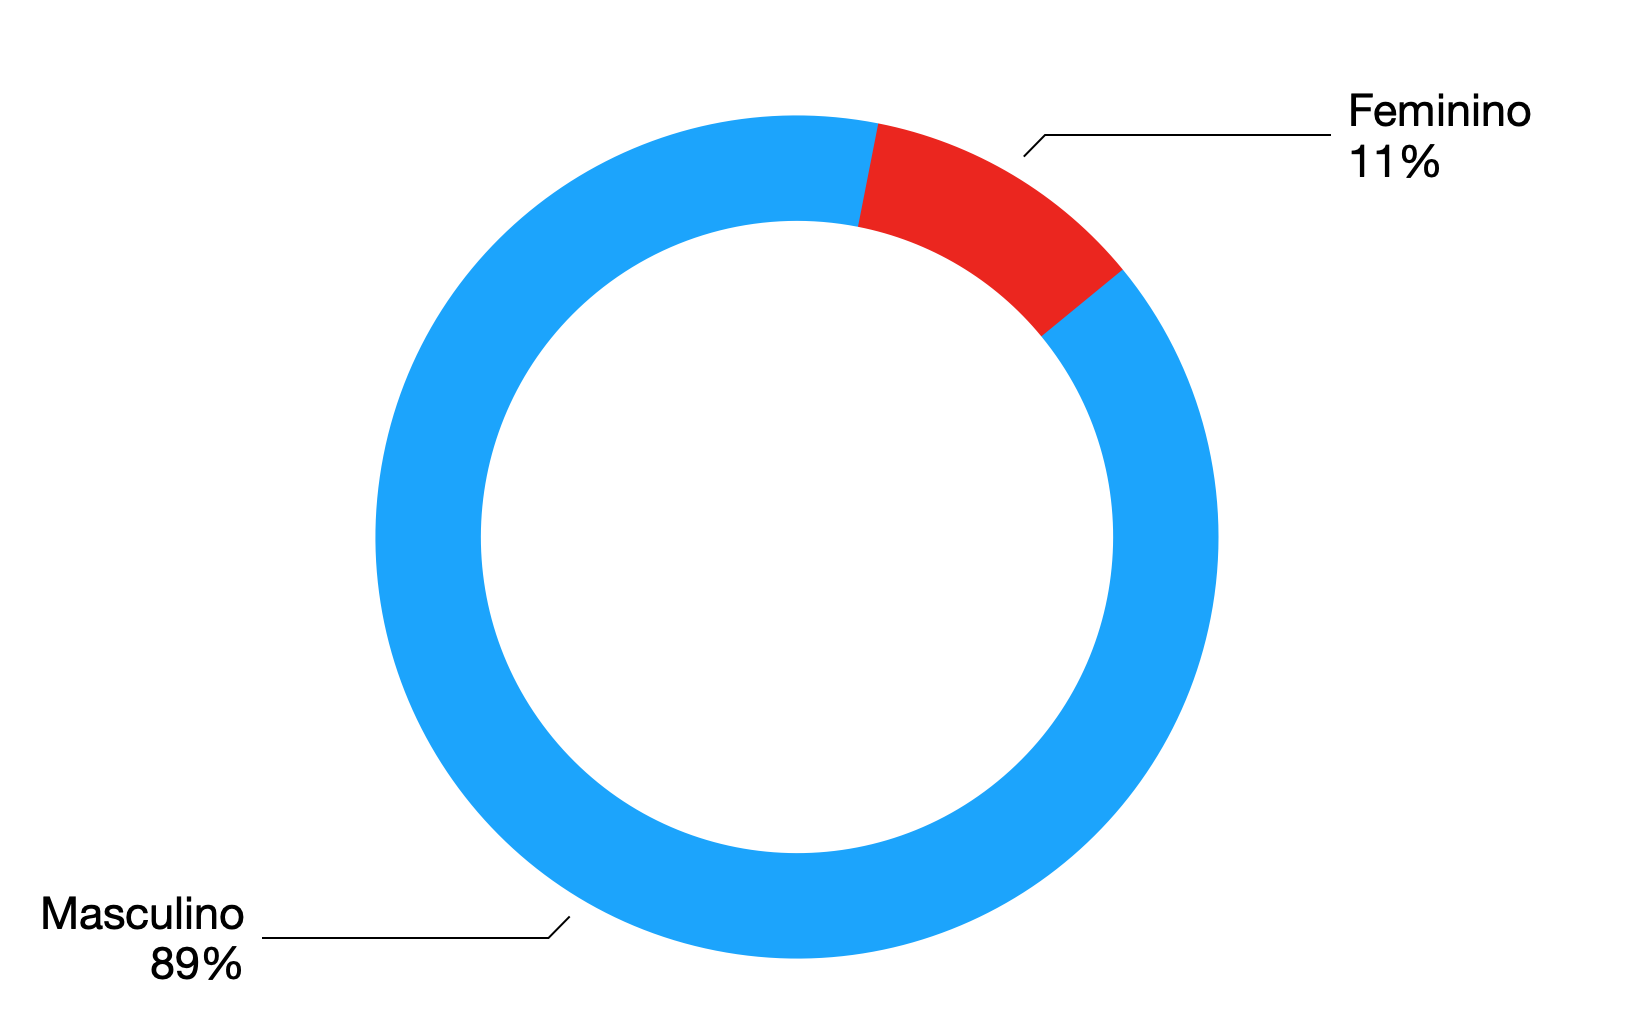
\includegraphics[width=5cm,height=3cm]{Quantidade de Homens e Mulheres.png}
    \caption{Categorias}
    \label{fig:my_label}
\end{figure}
Podemos ver que o UFC ainda é um esporte predominantemente masculino, pelo fato de apenas cerca de $10\%$ dos lutadores são mulheres.\\

Quando vamos analisar separando os sexos, notamos que a proporção de homens por categorias, segue distribuição padrão. Isso se deve pelo fato de existirem poucos homens nos extremos dos pesos, um reflexo da sociedade.\\

Enquanto nas mulheres isso não está tão claro, mas ao lembrarmos que em media o peso das mulheres é menor que o do homem, podemos notar que o gráfico referente ao das mulheres é a metade após a média da distribuição padrão feminina.\\

\begin{figure}[H]
\centering
\subfigure[Lutadores por Categoria\label\{]{
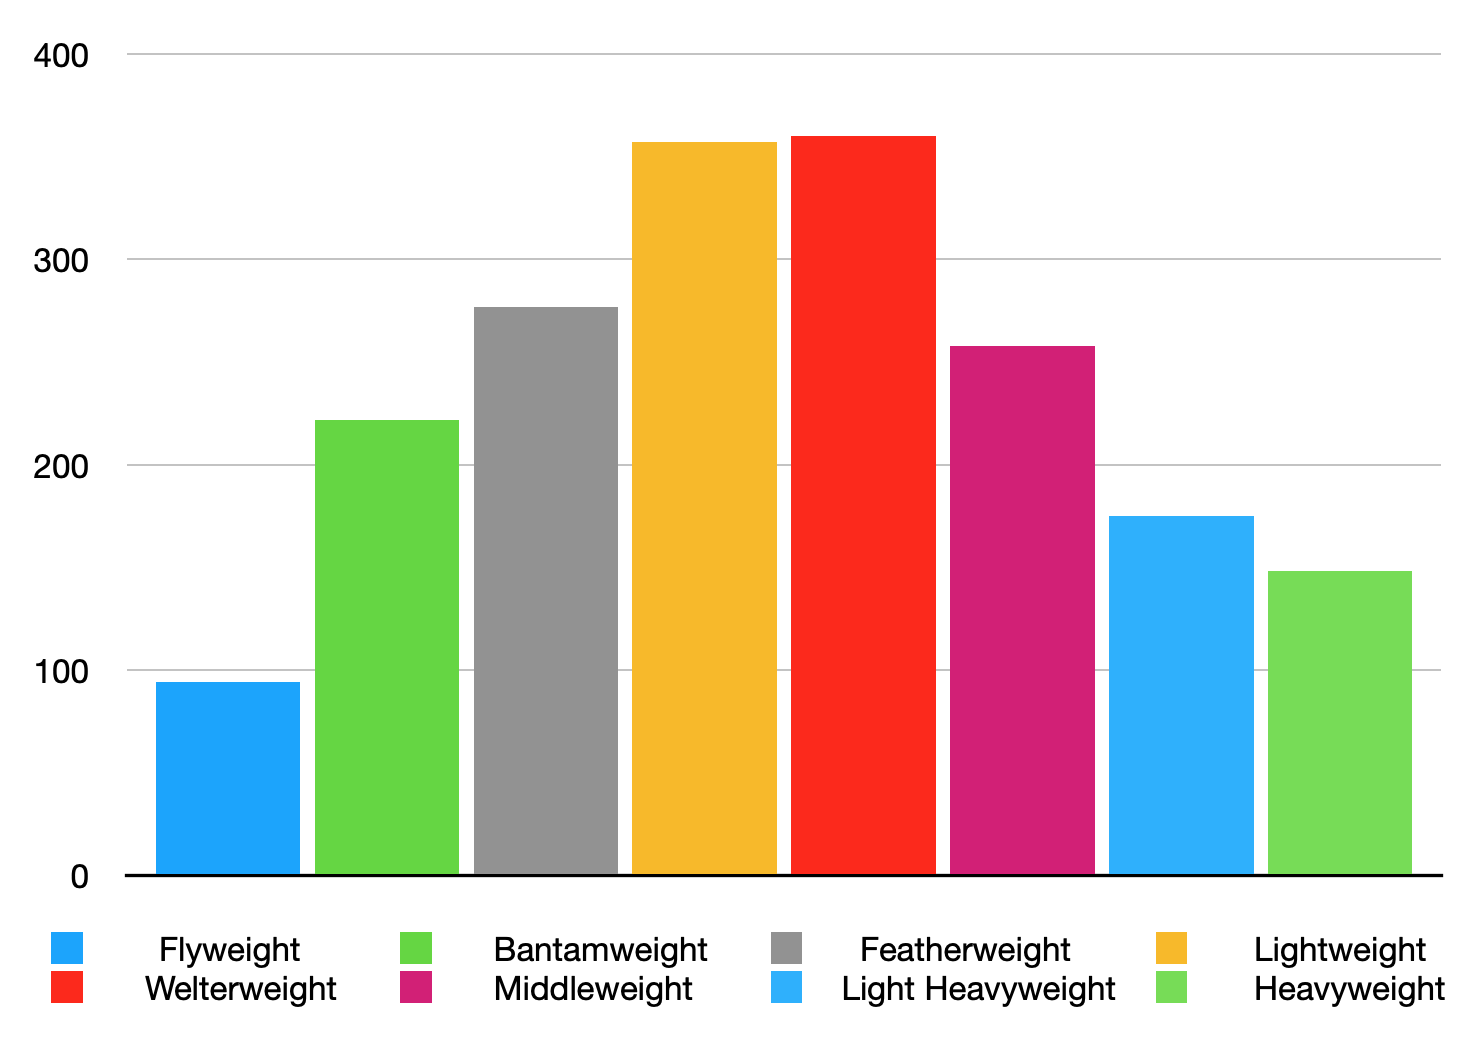
\includegraphics[width=7cm,height=4cm]{Lutadores por Categoria.png}}
\subfigure[Lutadoras por Categoria\label\{]{
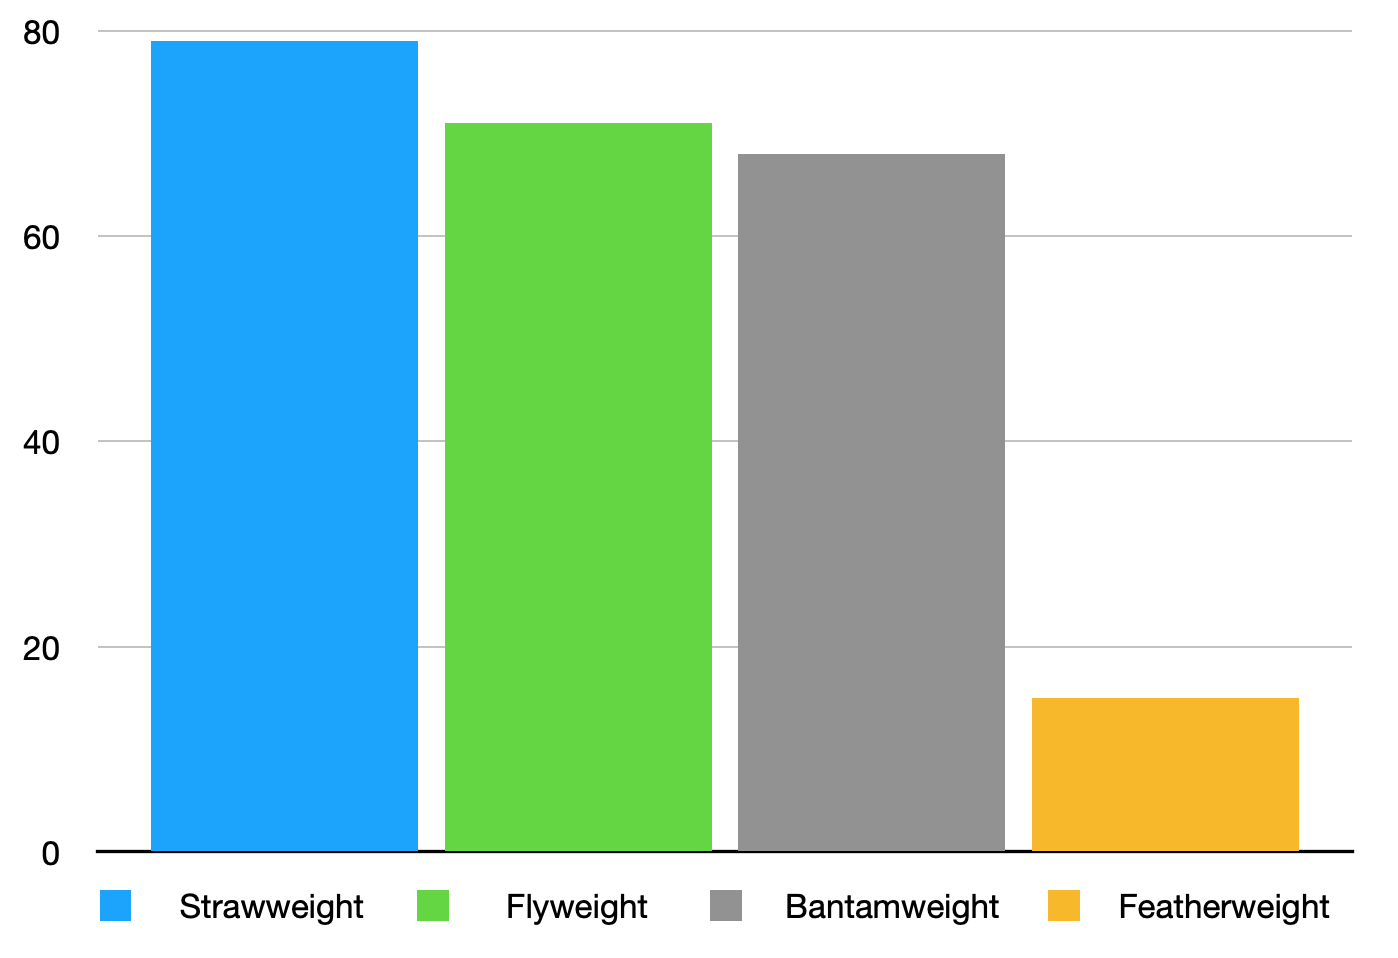
\includegraphics[width=4cm,height=4cm]{Lutadoras por Categoria.png}}
\end{figure}
\\

Quando comparamos as mesmas categorias de mulheres e homens, notamos que em nenhuma as mulheres estão mais presentes que os homens e que a categoria que mais tende a equidade é a \textit{Flyweight} que é a menos competida pelos homens e a mais competida pelas mulheres.\\

\begin{figure}[H]
    \centering
    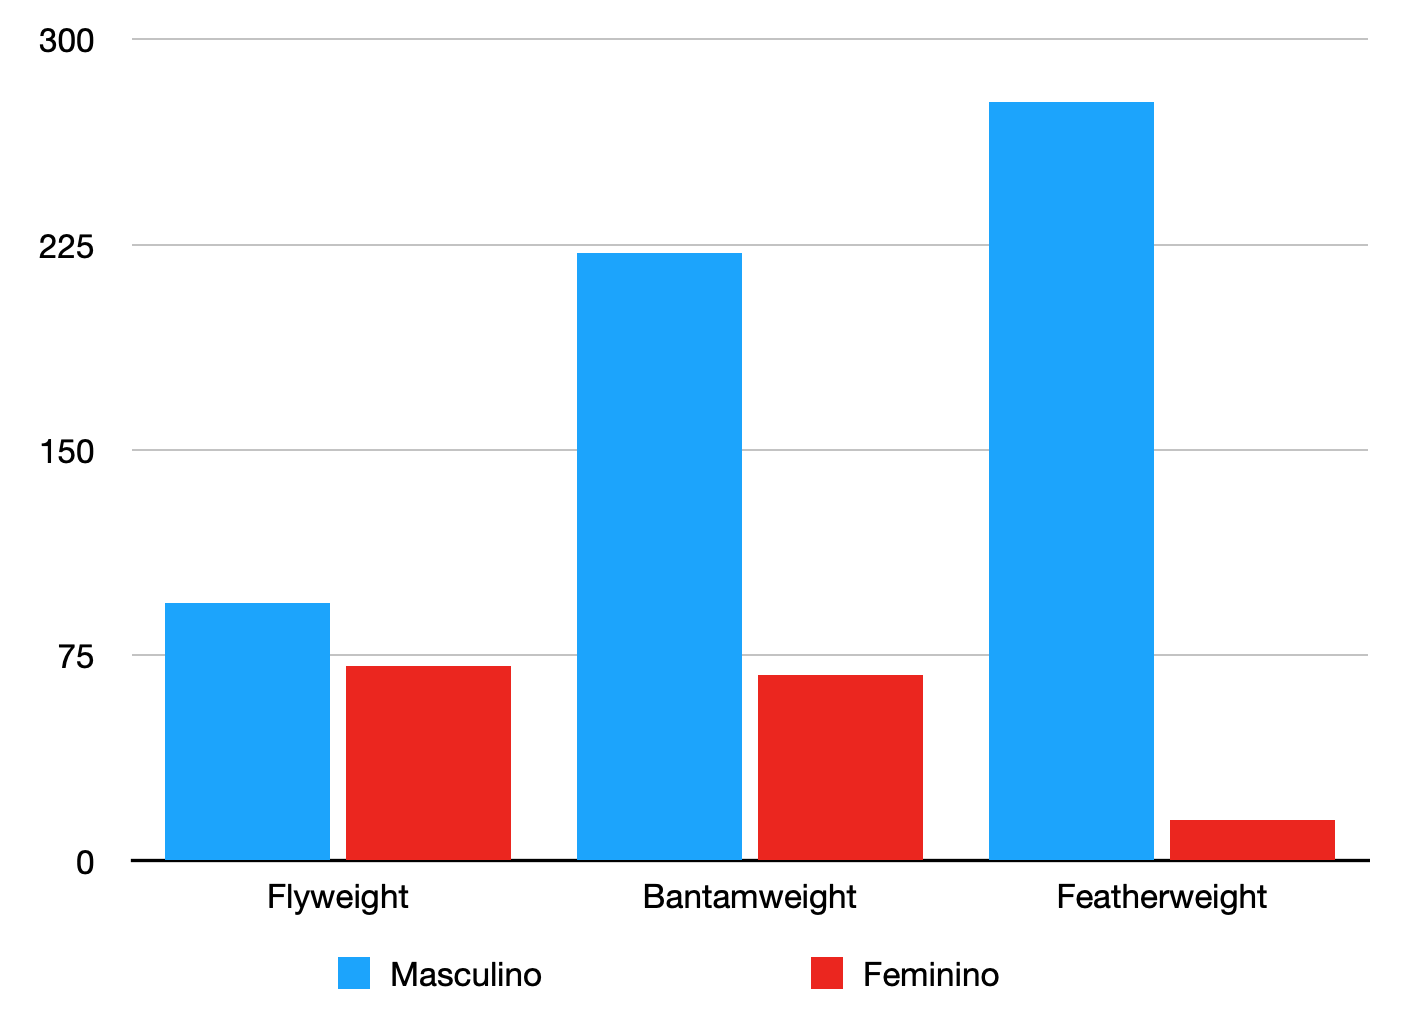
\includegraphics[width=5cm,height=4cm]{Comparação Quantidade de Lutadoras e Lutadores}
    \caption{Comparação Quantidade de Lutadoras e Lutadores}
    \label{fig:my_label}
\end{figure}

\textbf{2.}Como ocorre a distribuição por classe de peso? A diferença de classe muda a quantidade de lutas ?\\

As lutas disponíveis nos dados contam com nove categorias, na qual os homens disputam oito (todas com excessão da mais leve \textit{strawweight}) e as mulheres apenas quatro (sendo as mais leves). \\

\begin{figure}[H]
\centering
\subfigure[Categorias dos Homens\label\{]{
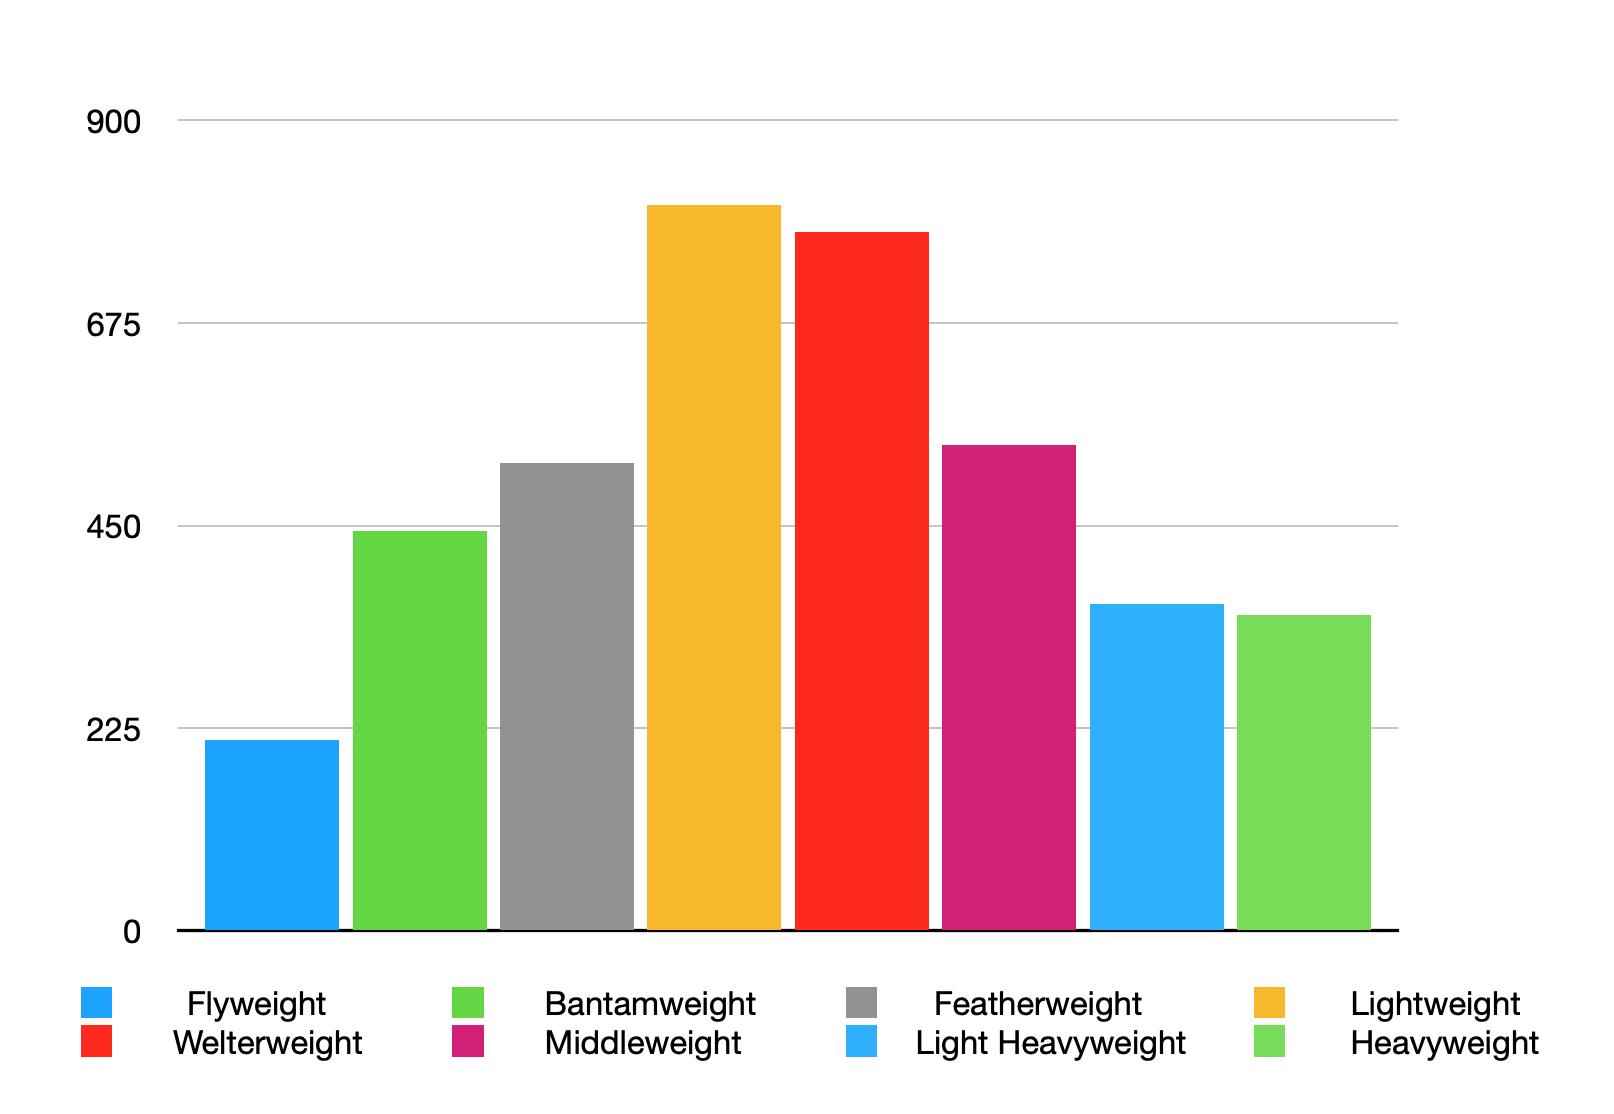
\includegraphics[width=7cm,height=4cm]{Categorias Homens.png}}
\subfigure[Categorias das Mulheres\label{}]{
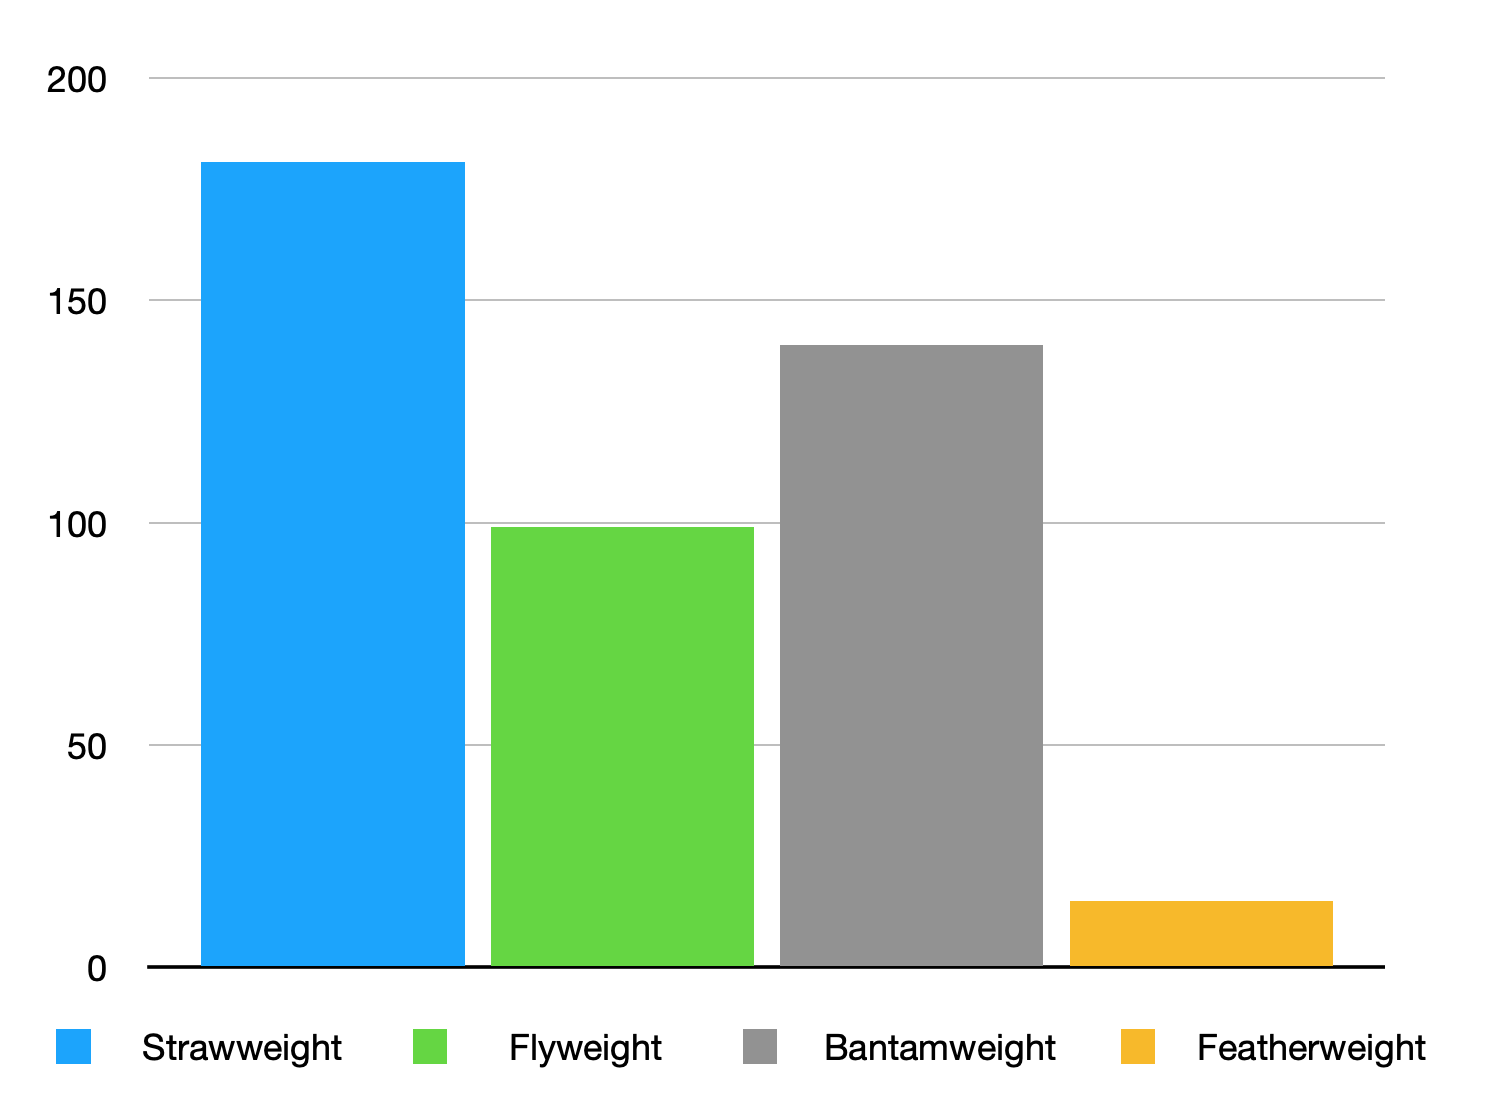
\includegraphics[width=4cm,height=4cm]{Categorias Mulheres.png}}
\end{figure} \\

Com base nos gráficos podemos ver que a distribuição de quantidades de lutas nas classes masculinas se aproximam da distribuição padrão. O que é muito relacionado com o fato de que a quantidade de homens por categoria também sejam distribuídos de forma padrão. \\

Já no das mulheres não vemos essa distribuição, o que é explicado pela baixa amostragem, comparado com a dos homens. Também vale notar que lutadoras que pertencem a categoria \textit{Flyweight} participam de menos lutas que as das categorias \textit{Bantamheight} e \textit{Strawweight}, vemos isso ao comparar esse gráfico com o de quantidade de lutadoras femininas.\\

O próximo gráfico representa as quantidades de lutas por categorias unindo as femininas e masculinas.\\

\begin{figure}[H]
    \centering
    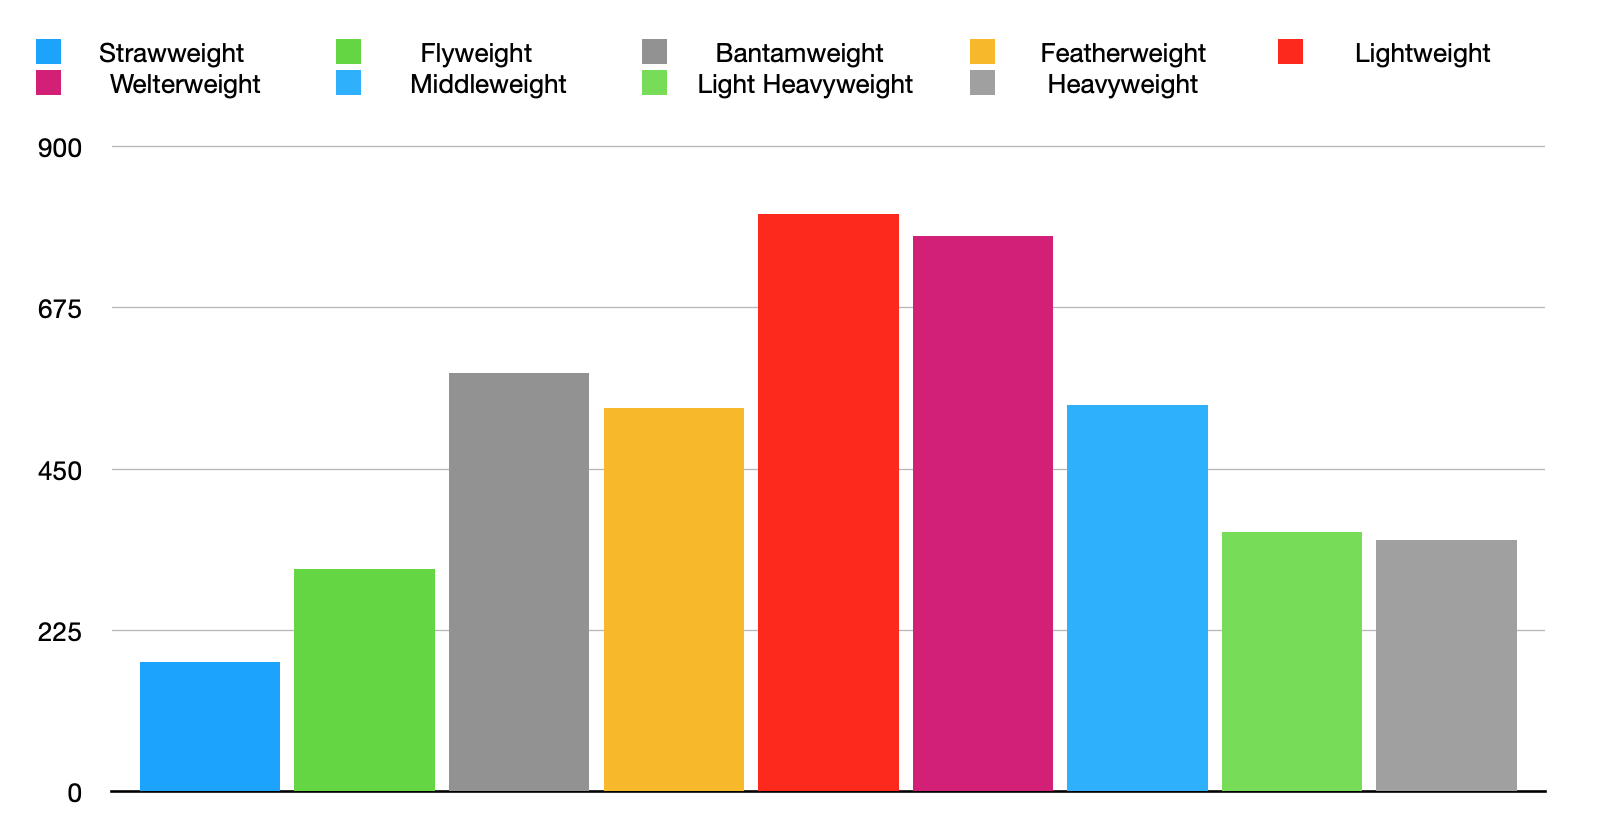
\includegraphics[width=8cm,height=4cm]{Categorias.png}
    \caption{Categorias}
    \label{fig:my_label}
\end{figure}
\\
Percebesse que quando unimos os dois sexos se mantêm a distribuição padrão, diminuindo o erro causado pelas poucas lutas femininas.\\

\newpage
\textbf{3.} Resultados das Lutas (Decision,TKO,Submission,KO).
\begin{figure}[H]
    \centering
    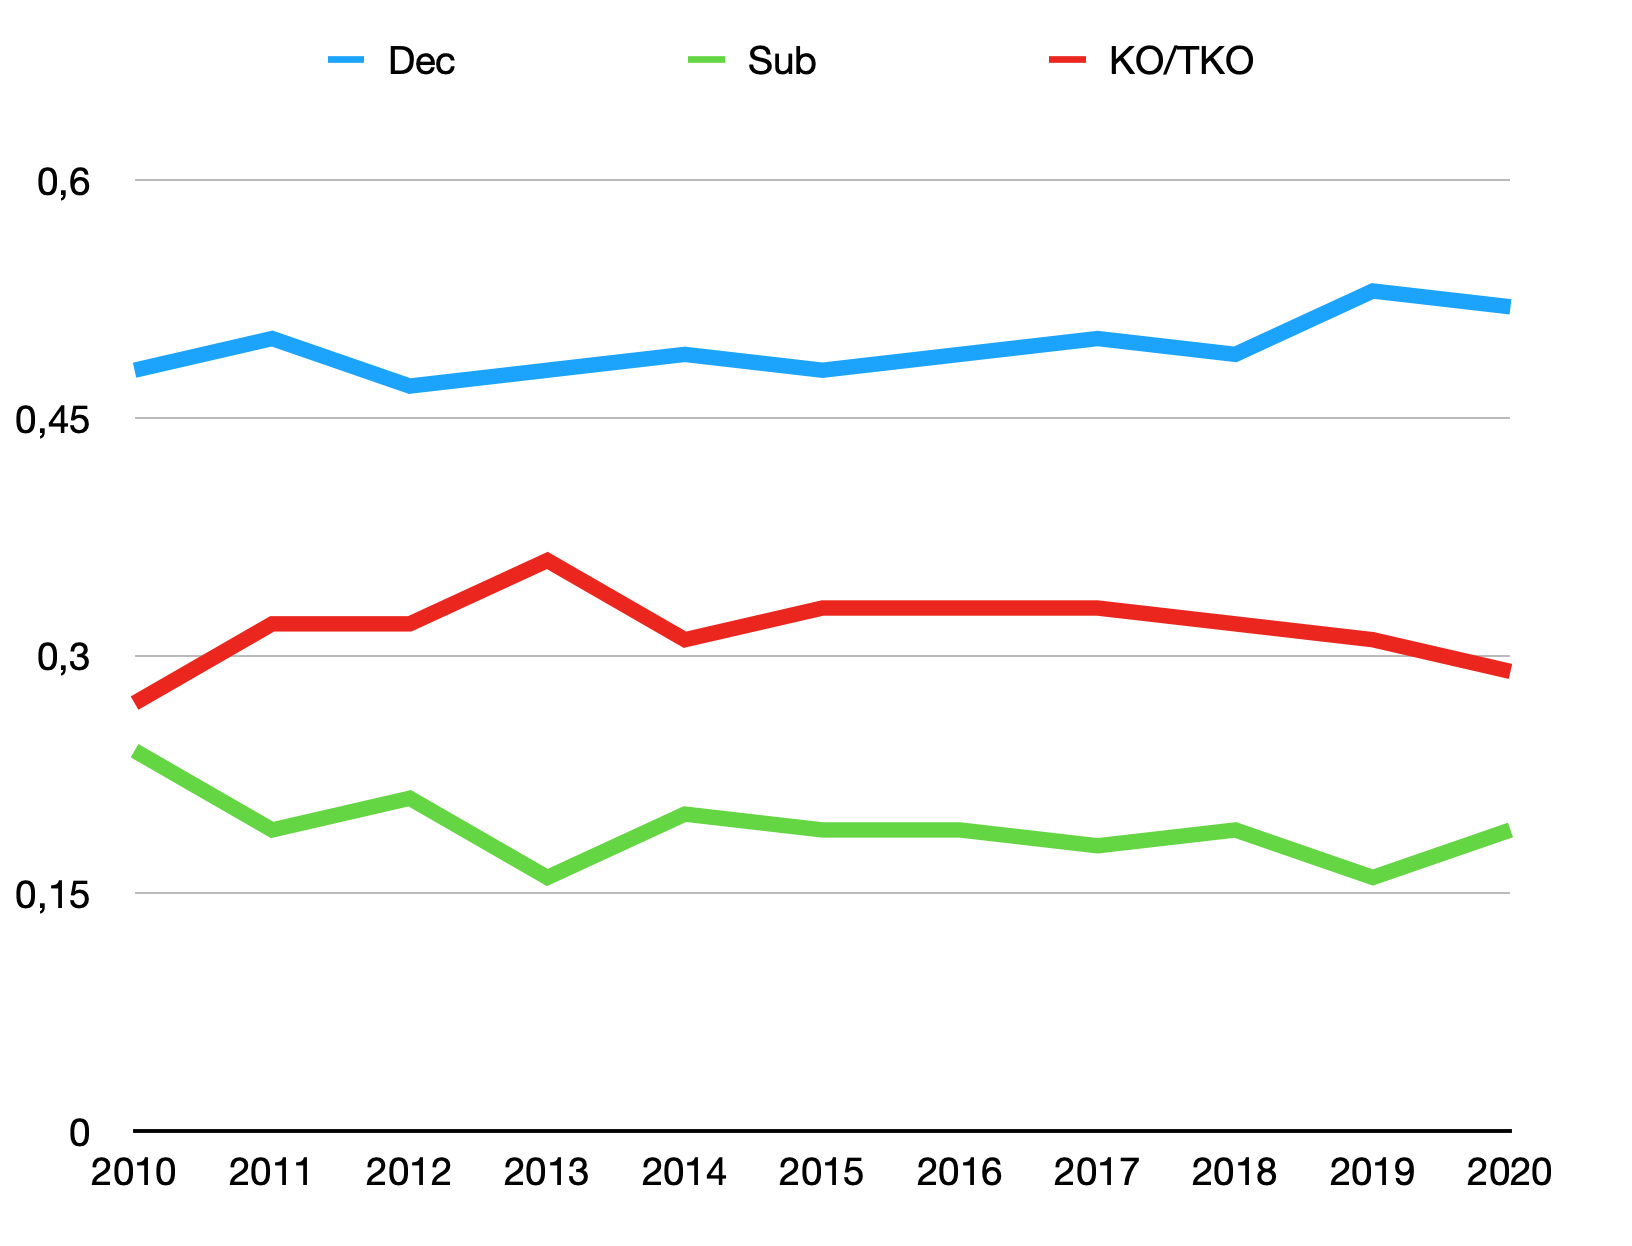
\includegraphics[width=8cm,height=4cm]{Final de Lutas.png}
    \caption{Final de Lutas.png}
    \label{fig:my_label}
\end{figure}
Vemos que em todos os anos a maior parte das lutas foi terminada por \textit{Decision}, que é quando a luta se prolonga por muito tempo e o juiz que decide quem foi o vencedor.  Depois vem as partidas que terminam em \textit{KO},  um dado alarmante para os lutadores, pois a chance de levarem um Nocaute chega a $30\% $ e por último imobilizações, que seria a vitoria mais "tranquila".\\

\textbf{4.} Distribuição de Quantidades de Vitórias.
\begin{figure}[H]
\centering
\subfigure[Distribuição por Vitórias Masculino\label\{]{
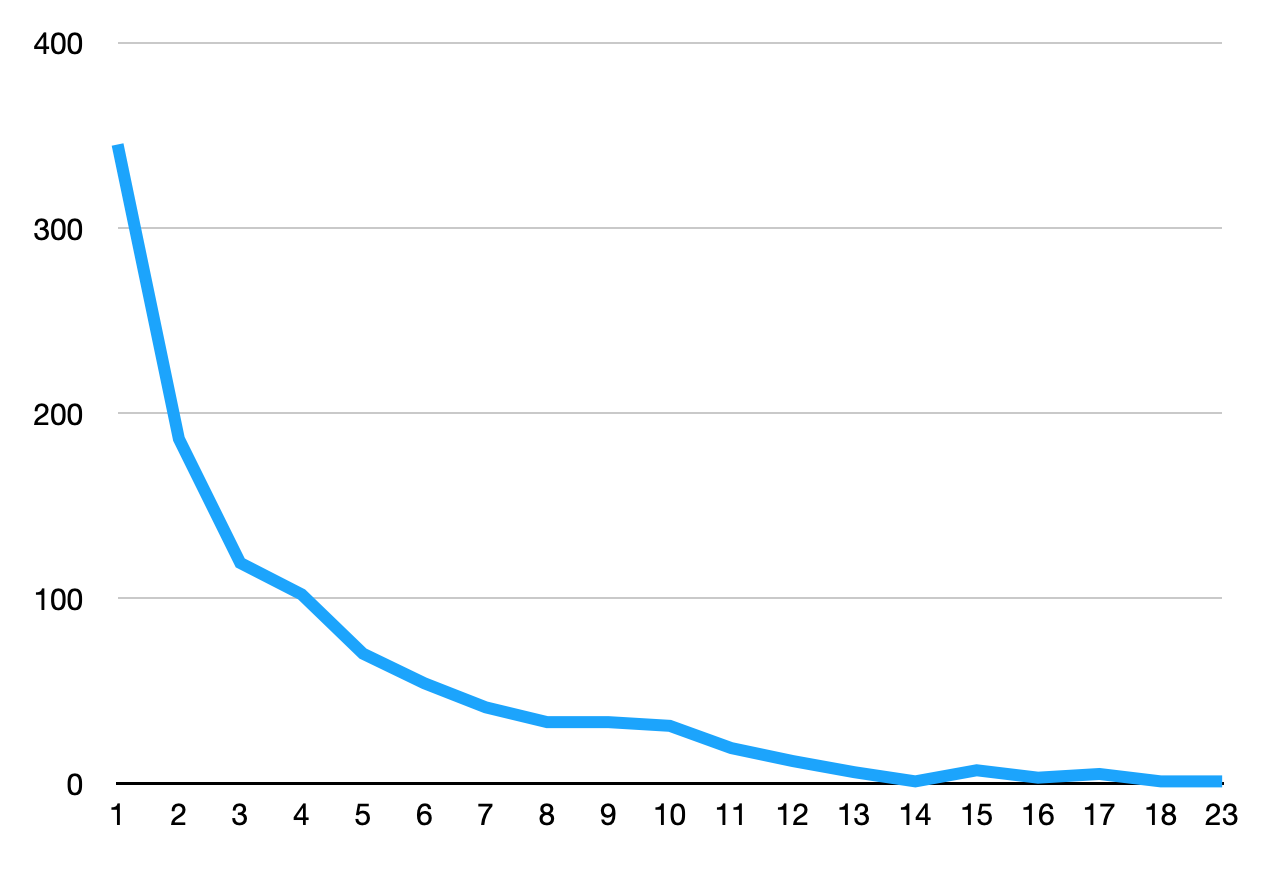
\includegraphics[width=5cm,height=3cm]{Distribuição por Vitórias Masculino.png}}
\subfigure[Distribuição por Vitórias Feminino\label{}]{
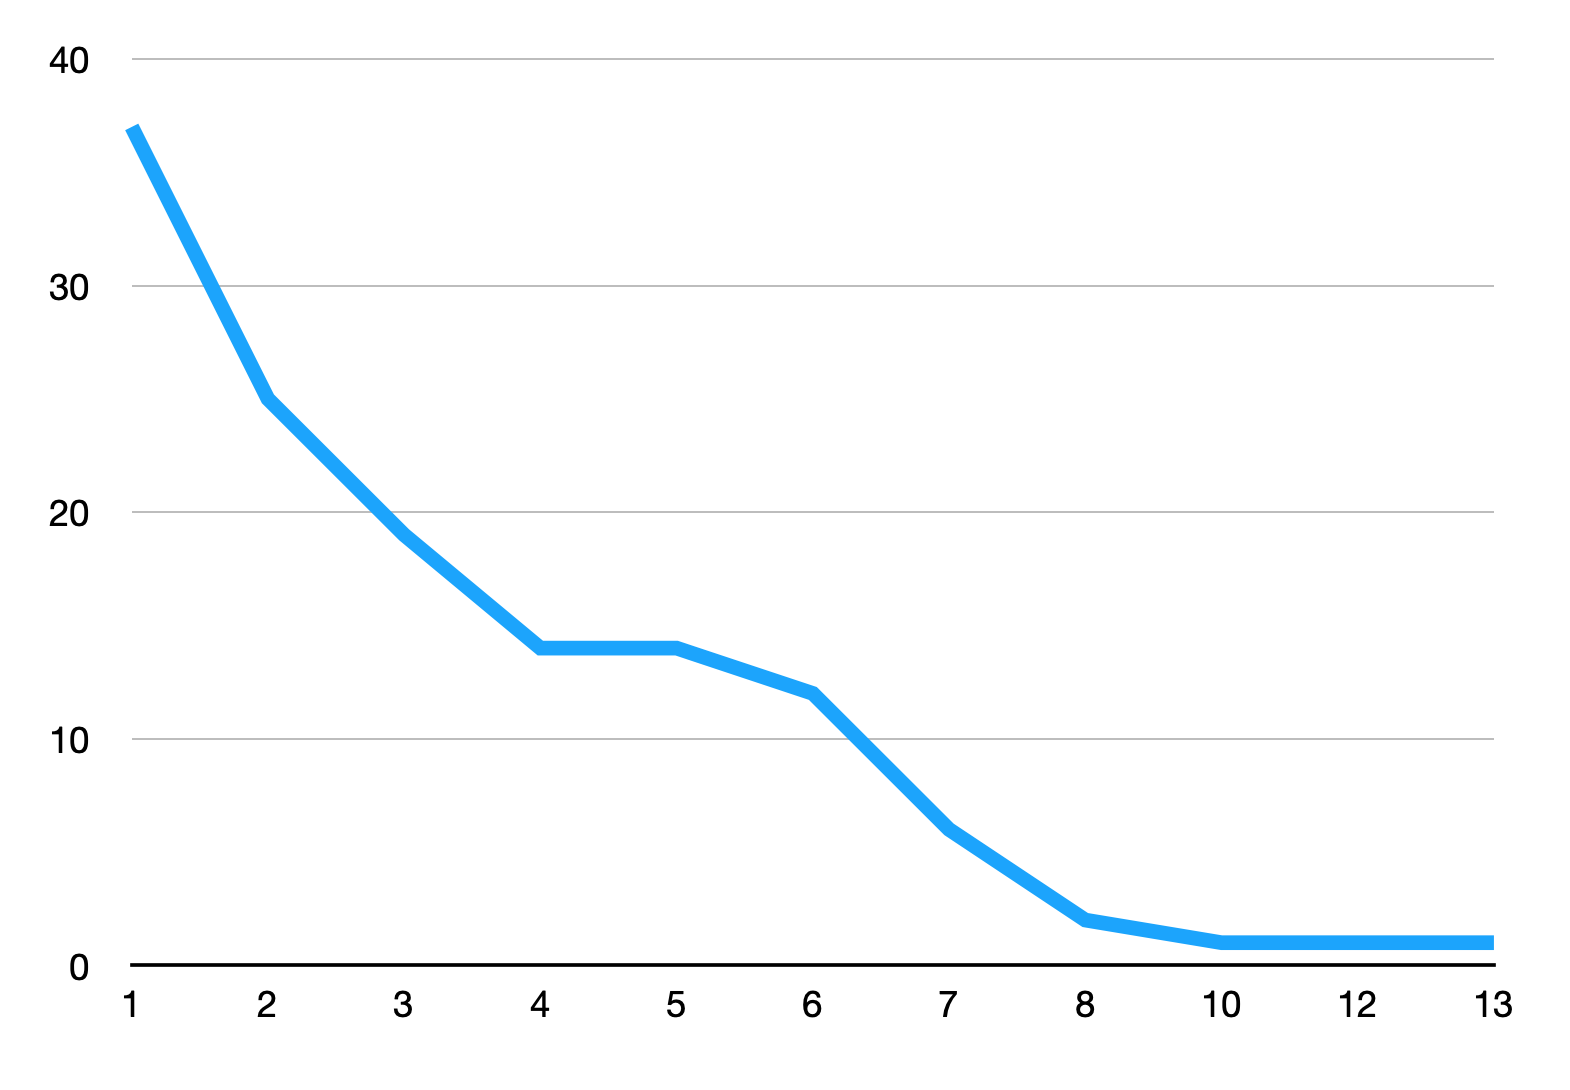
\includegraphics[width=5cm,height=3cm]{Distribuição por Vitórias Feminino.png}}
\end{figure} \\
Fica claro através do gráfico que a distribuição por vitorias segue a distribuição de Paretto, visto que as vitórias podem ser descritas pelo "Rich gets Richer" pois se um jogador esta ganhando muitas,  nos leva a pensar que ele é bom, logo vai continuar ganhando. E o mesmo serve para quem perde muitas.\\

\newpage
\textbf{5.} Relação Quantidade de Disputas e de Vitórias\\

\begin{figure}[H]
\centering
\subfigure[Top 10 das Vitórias Masculinas\label\{]{
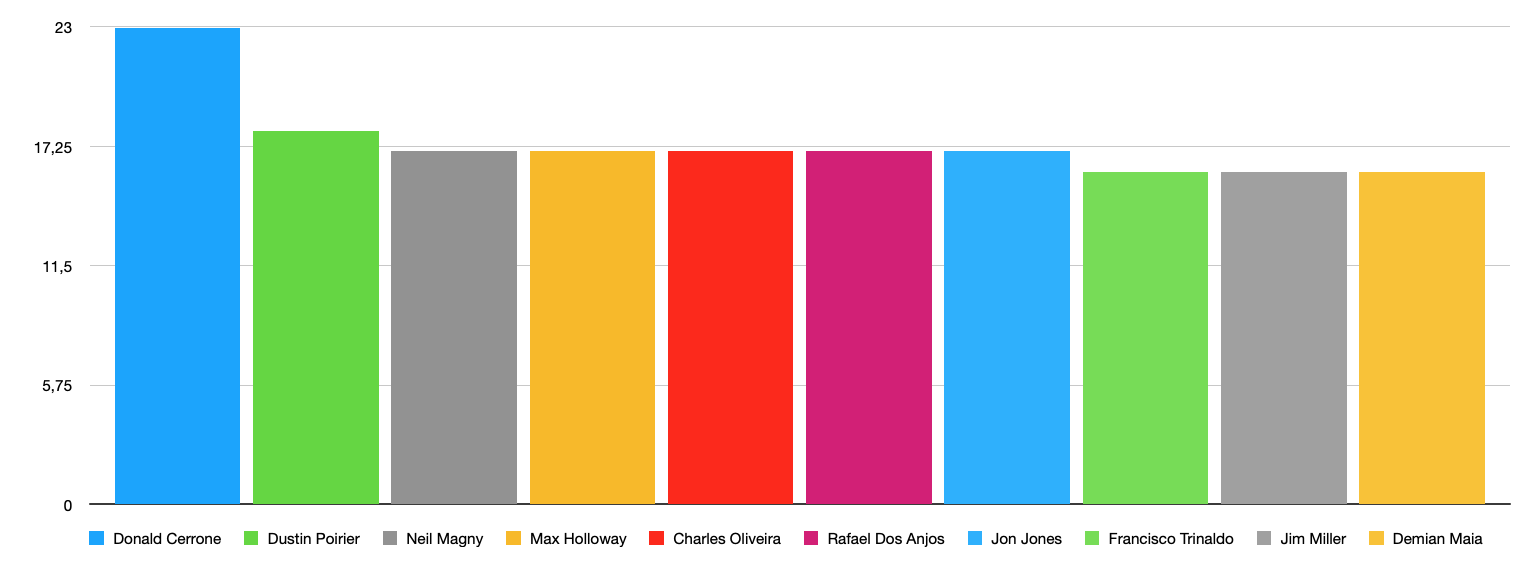
\includegraphics[width=10cm,height=4cm]{Top 10 das Vitórias Masculinas}}
\subfigure[Top 10 das Disputas Masculinas\label{}]{
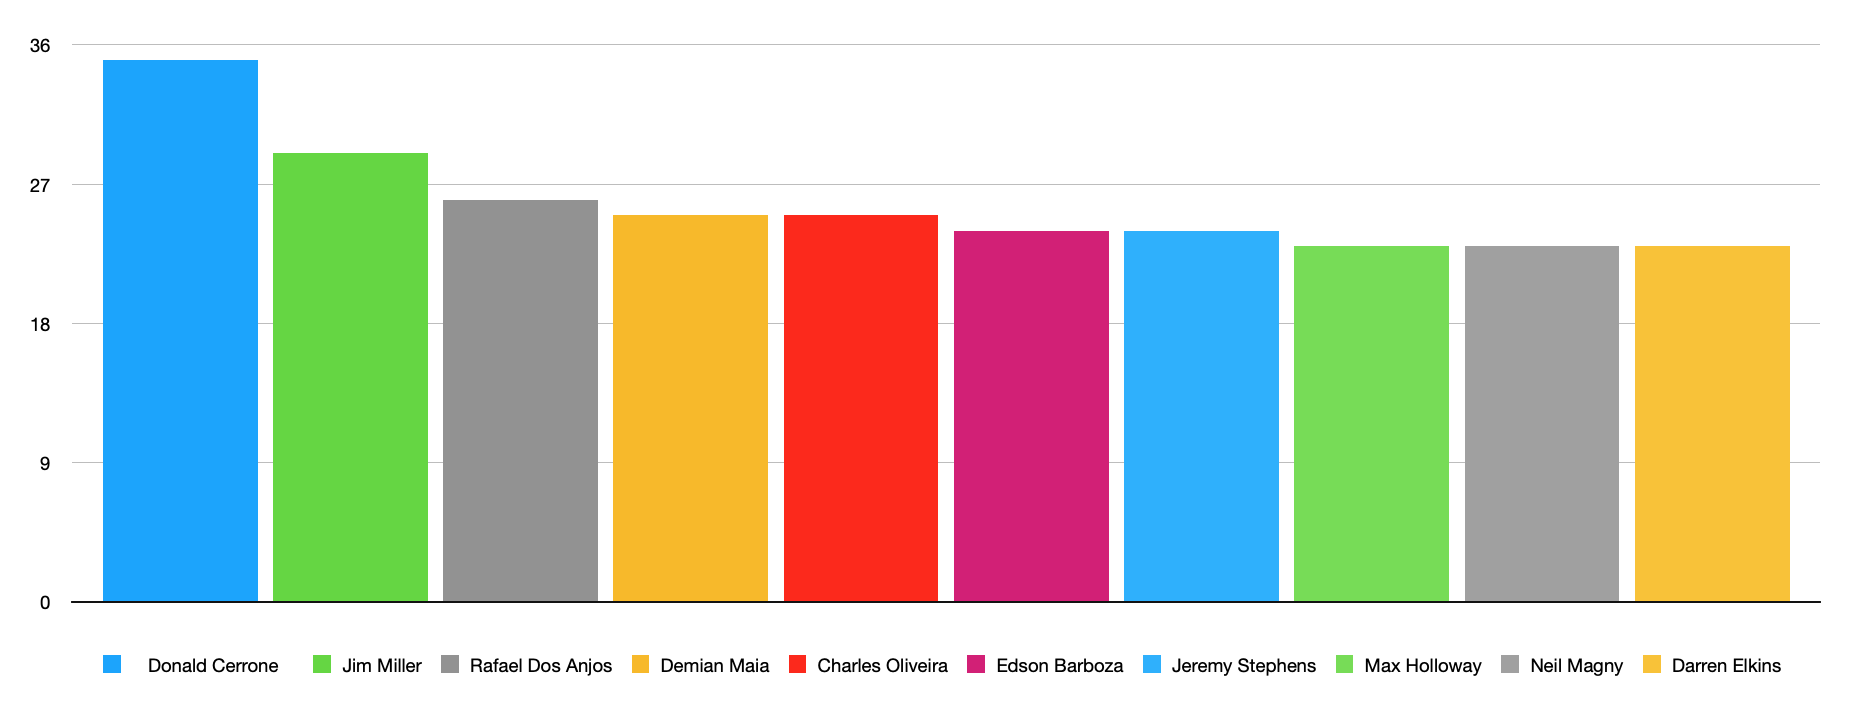
\includegraphics[width=10cm,height=4cm]{Top 10 das Disputas Masculinas.png}}
\end{figure} \\

Podemos achar a primeira vista que o jogador que mais acumulou vitórias em sua carreira é o melhor lutador, porém essa premissa não é verdadeira. Podemos ver que \textit{Donald Cerrone} possui o maior número de vitórias assim como o de disputas. Mas se calcularmos a sua porcentagem de vitória ele já sai da primeira colocação $(0,657)$ e quem assume é \textit{Dustin Poirier} $ (0,782 )$. Logo se quisermos comparar lutadores de uma forma simples mas com um respaldo significativo basta vermos a porcentagem de vitórias por partidas disputadas.\\

\newpage
\textbf{6.} Relação de Torcida com Resultado da Luta
\begin{figure}[H]
    \centering
    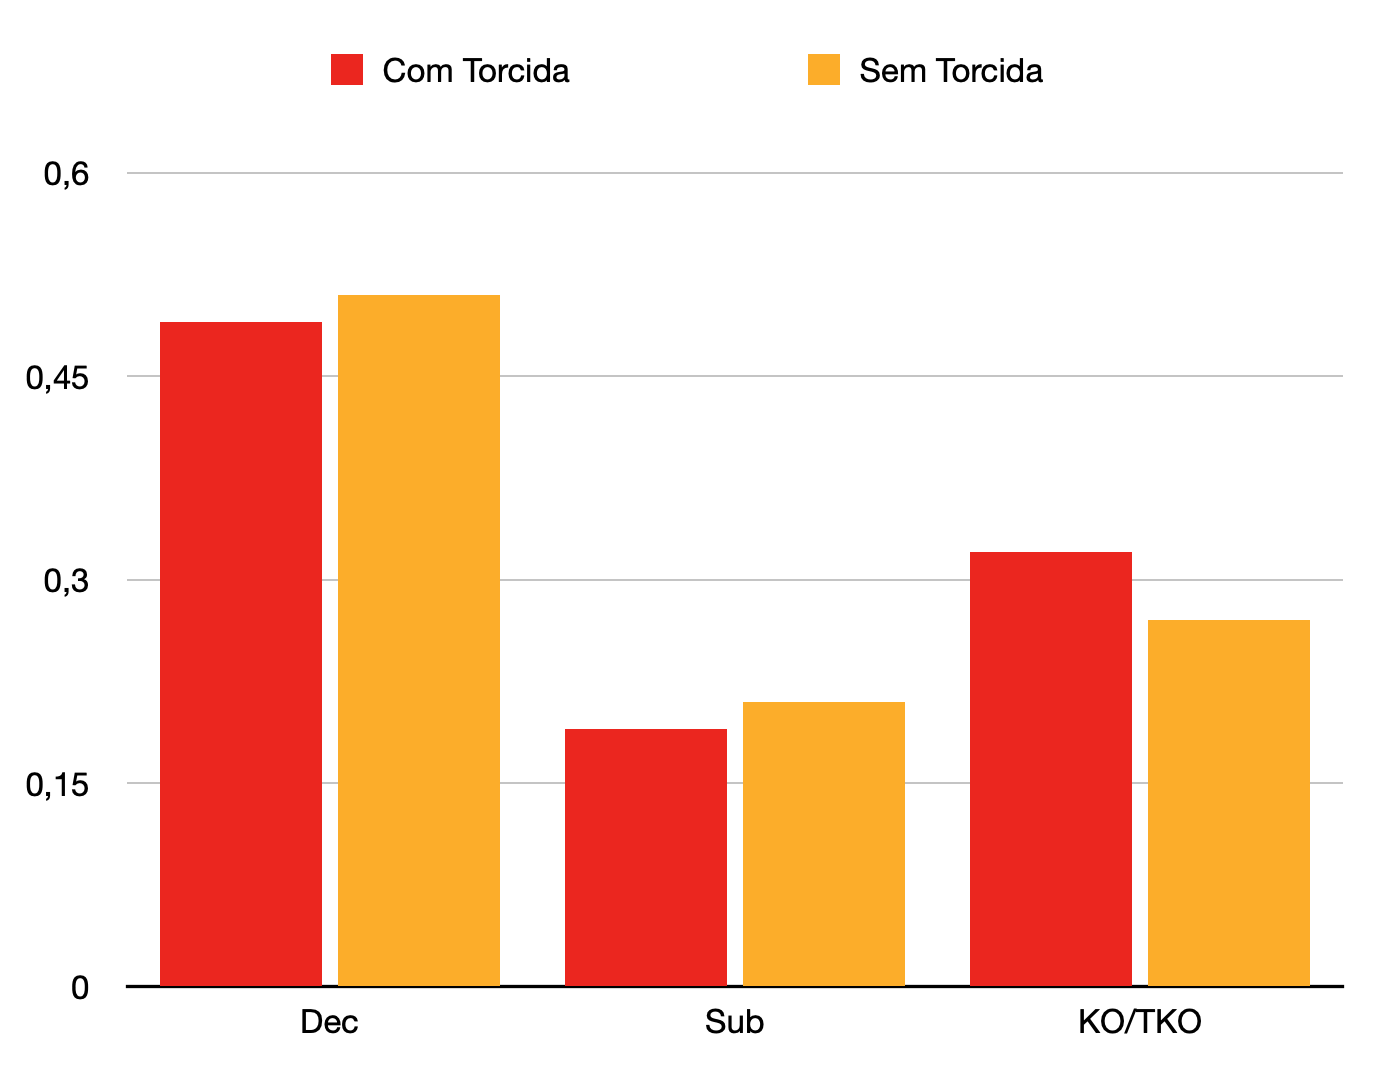
\includegraphics[width=7cm,height=4cm]{Relação Torcida e Resultado.png}
    \caption{Relação Torcida e Resultado}
    \label{fig:my_label}
\end{figure}

Vemos que quando não há torcida temos um número maior de \textit{Decision} e quando há ocorre um aumento no número de \textit{KO/TKO}.Nos levando a supor que a presença da torcida incentiva  o lutador a agir de forma mais agressiva, assim influenciando um número de Nocautes. \\

\textbf{7.} Relação da Cor do Lutador e Resultado

\begin{figure}[H]
    \centering
    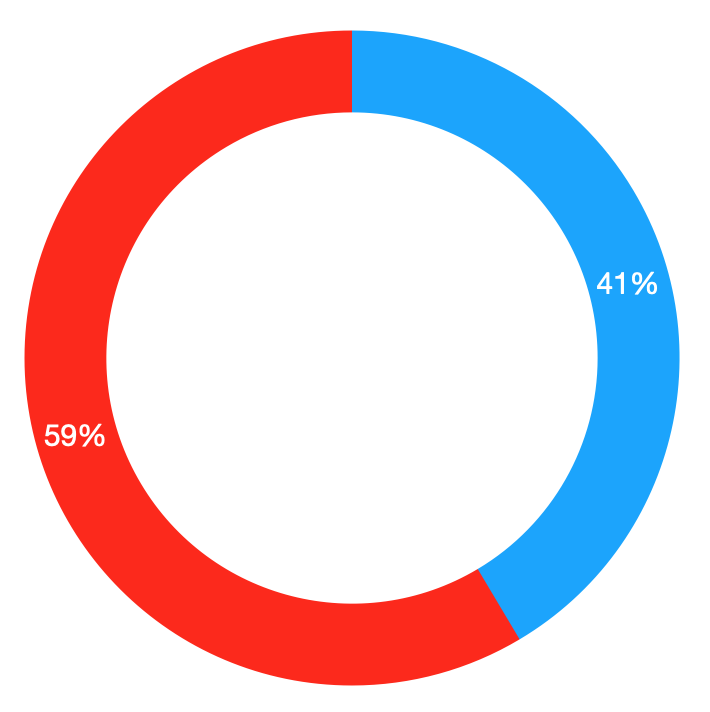
\includegraphics[width=3cm,height=3cm]{Cor dos Lutadores.png}
    \caption{Cor dos Lutadores}
    \label{fig:my_label}
\end{figure}

Vemos um resultado diferente do esperado que seria uma tendencia ao meio ao meio. Isso é explicado pois aparentemente os lutadores favoritos ficam com a cor vermelha, porque sua posição fica de frente para as câmeras da luta. Outro boato que se conta é que normalmente na primeira partida de um lutador ele pega o azul. Esses seriam alguns dos fatores que mostram o porque dessa divergência de cinquenta porcento.\\

\newpage
\section{FIFA}
\subsection{Resultado de Análises}

\textbf{1.} Distribuição de Jogadores por Nacionalidade
\begin{figure}[H]
    \centering
    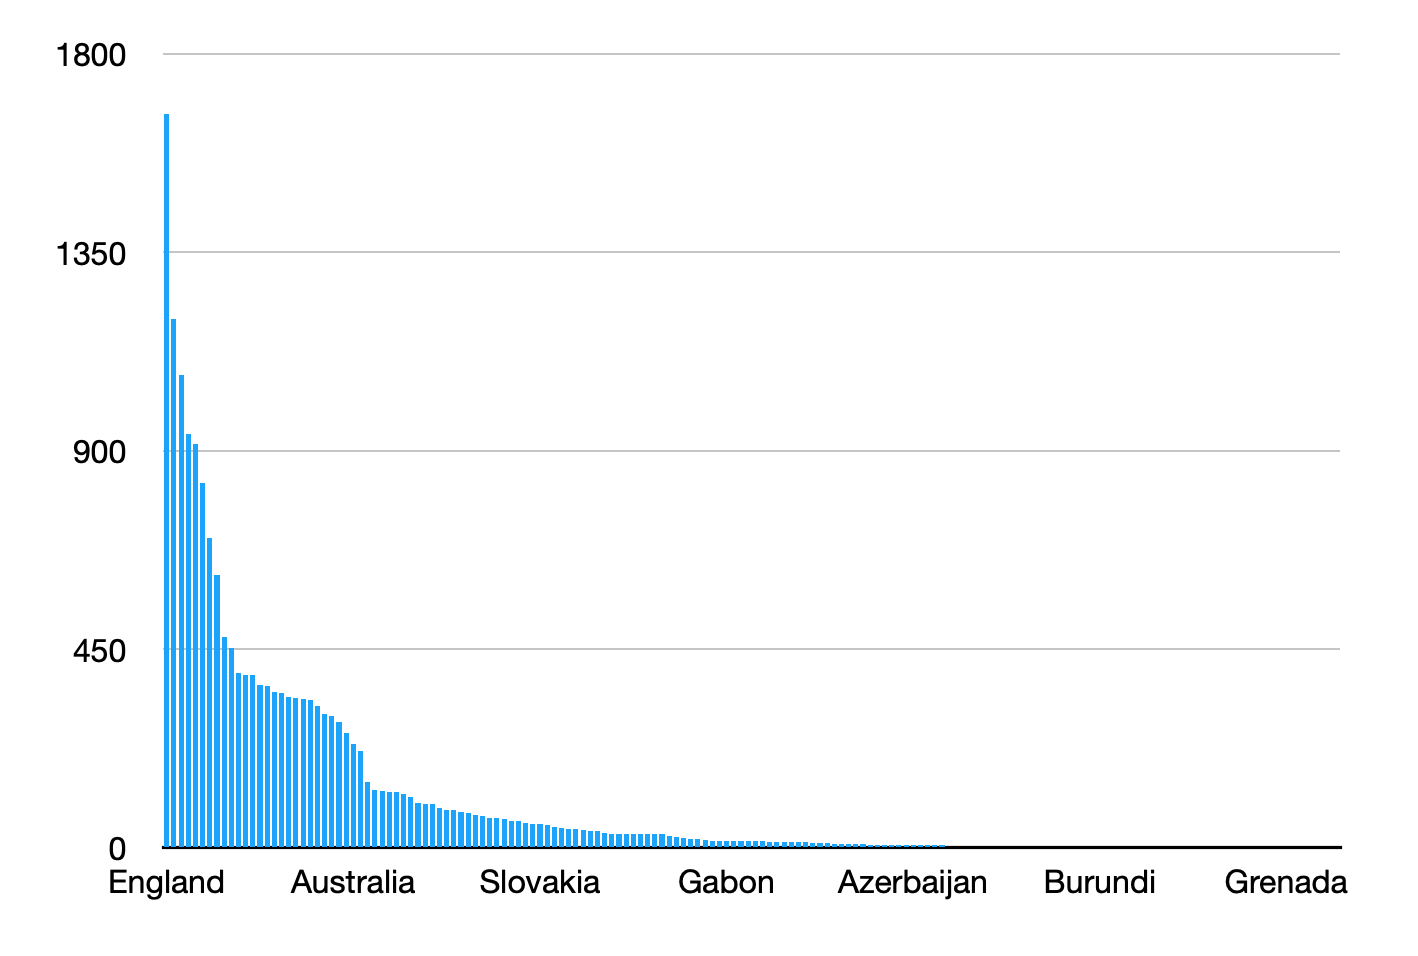
\includegraphics[width=10cm,height=5cm]{Distribuição de Jogadores por Nacionalidade.png}
    \caption{Distribuição de Jogadores por Nacionalidade}
    \label{fig:my_label}
\end{figure}
\begin{figure}[H]
    \centering
    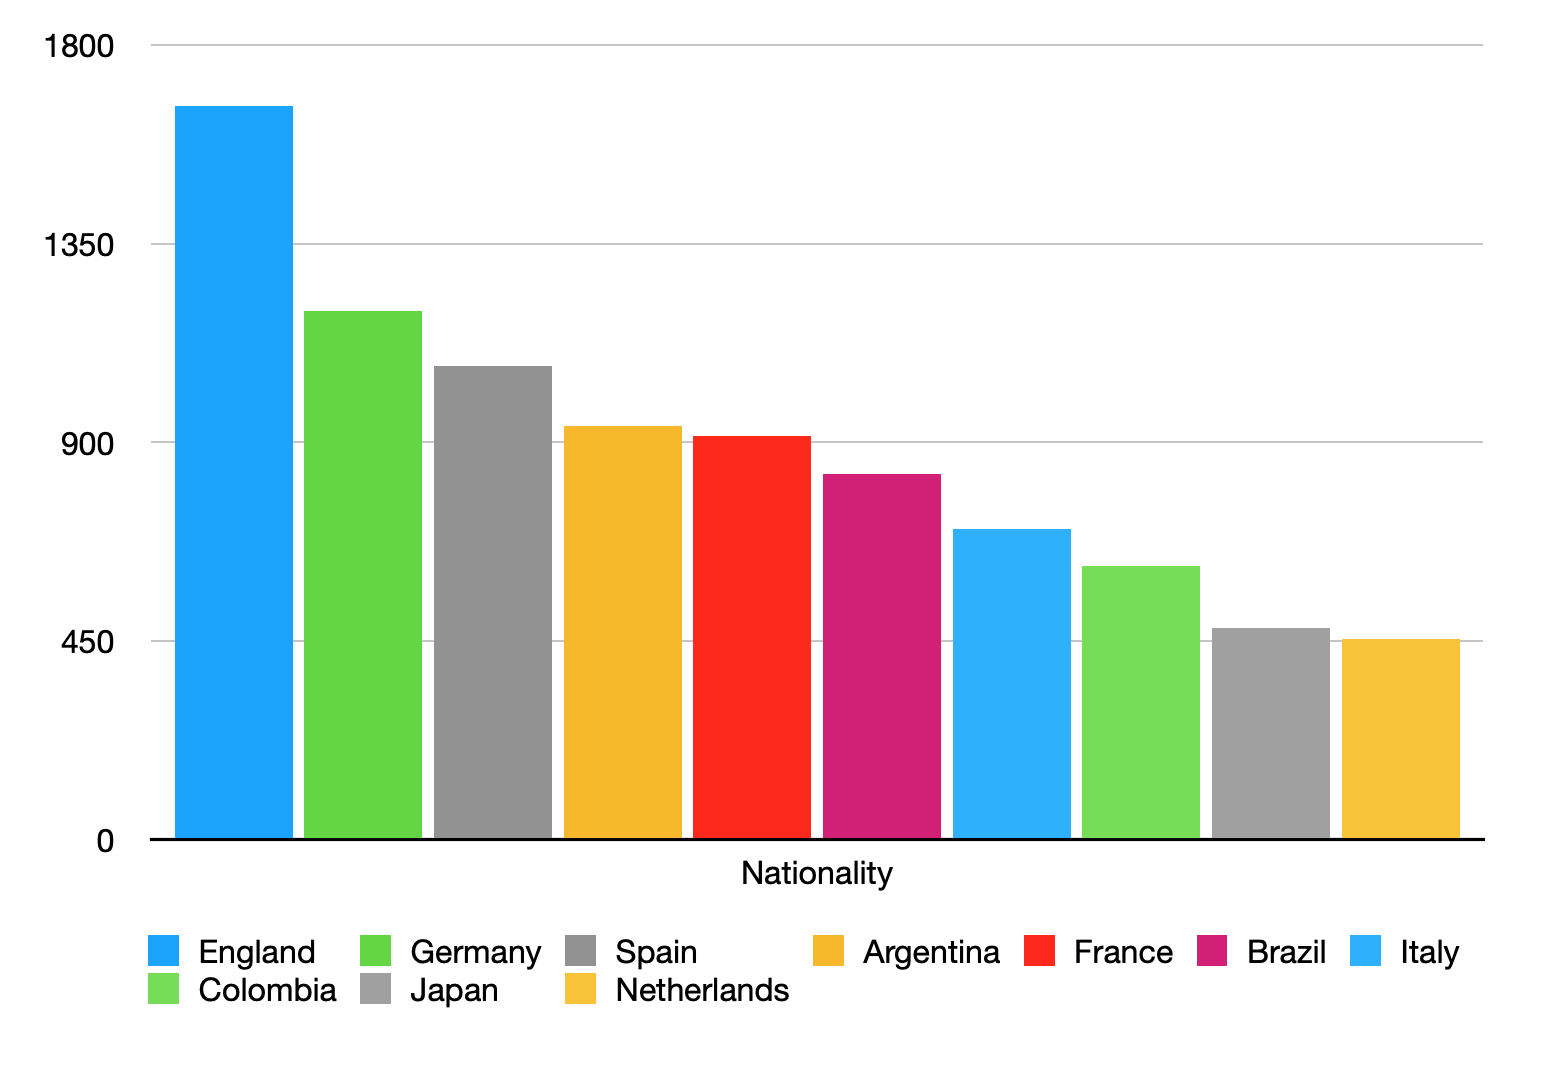
\includegraphics[width=10cm,height=5cm]{Top 10 Jogadores em Nacionalidade.png}
    \caption{Top 10 Jogadores em Nacionalidade}
    \label{fig:my_label}
\end{figure}

Podemos ver que distribuição de jogadores por nacionalidade segue com bastante fidelidade e distribuição de Pareto. E ao analisarmos os países que mais tem jogadores, vemos que não é uma coincidência que estão no topo justamente os maiores campeões da Copa do Mundo. Isso acontece pela cultura futebolística presente a anos nesses países.\\

\newpage
\textbf{2.} Somatório Médio de Overall dos Jogadores por Time

\begin{figure}[H]
    \centering
    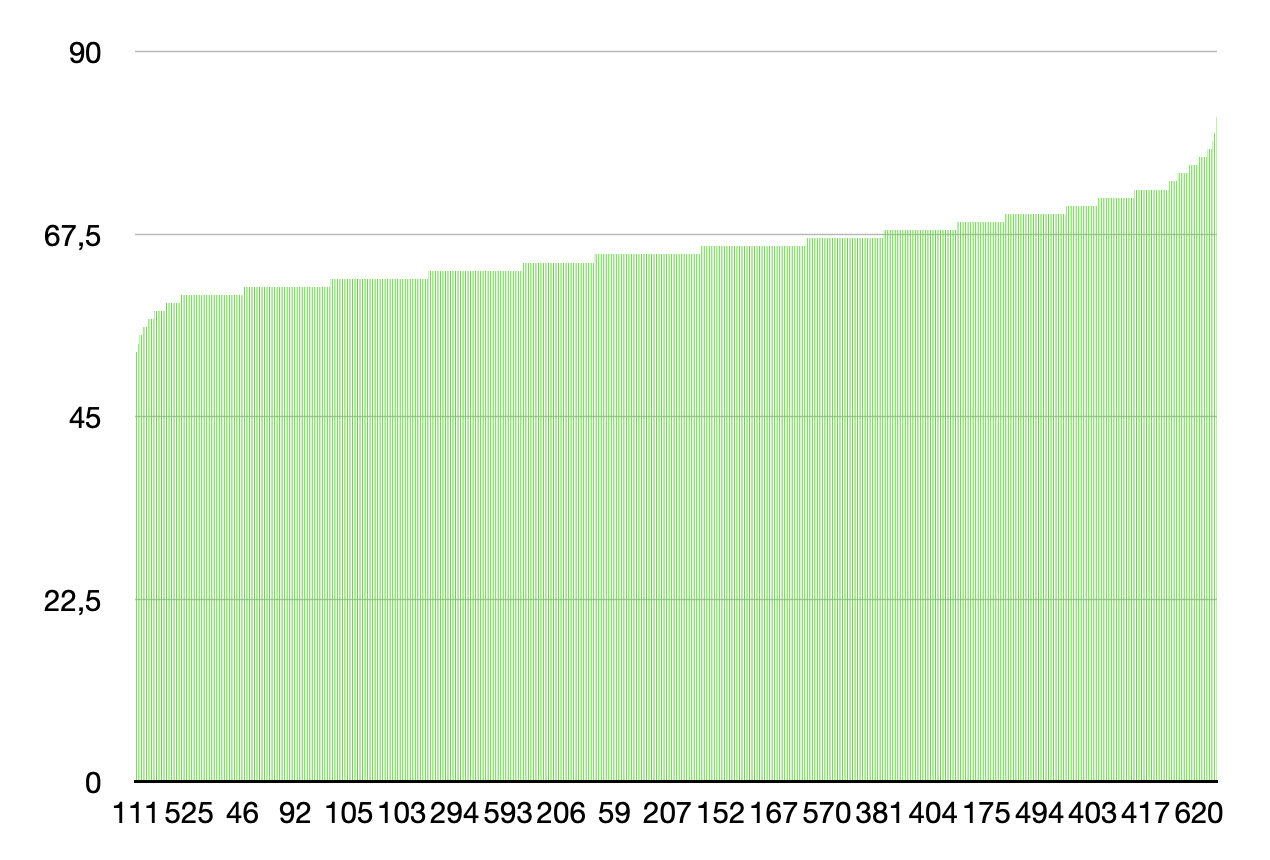
\includegraphics[width=6cm,height=4cm]{Overall dos Times.png}
    \caption{Overall dos Times}
    \label{fig:my_label}
\end{figure}

Podemos ver que pouquíssimos times estão nas extremidades e grande parte de encontra na média. Se  mudarmos a visualização do gráfico para contarmos a quantidade de times presentes nos intervalos de valores de Overall temos:
\begin{figure}[H]
    \centering
    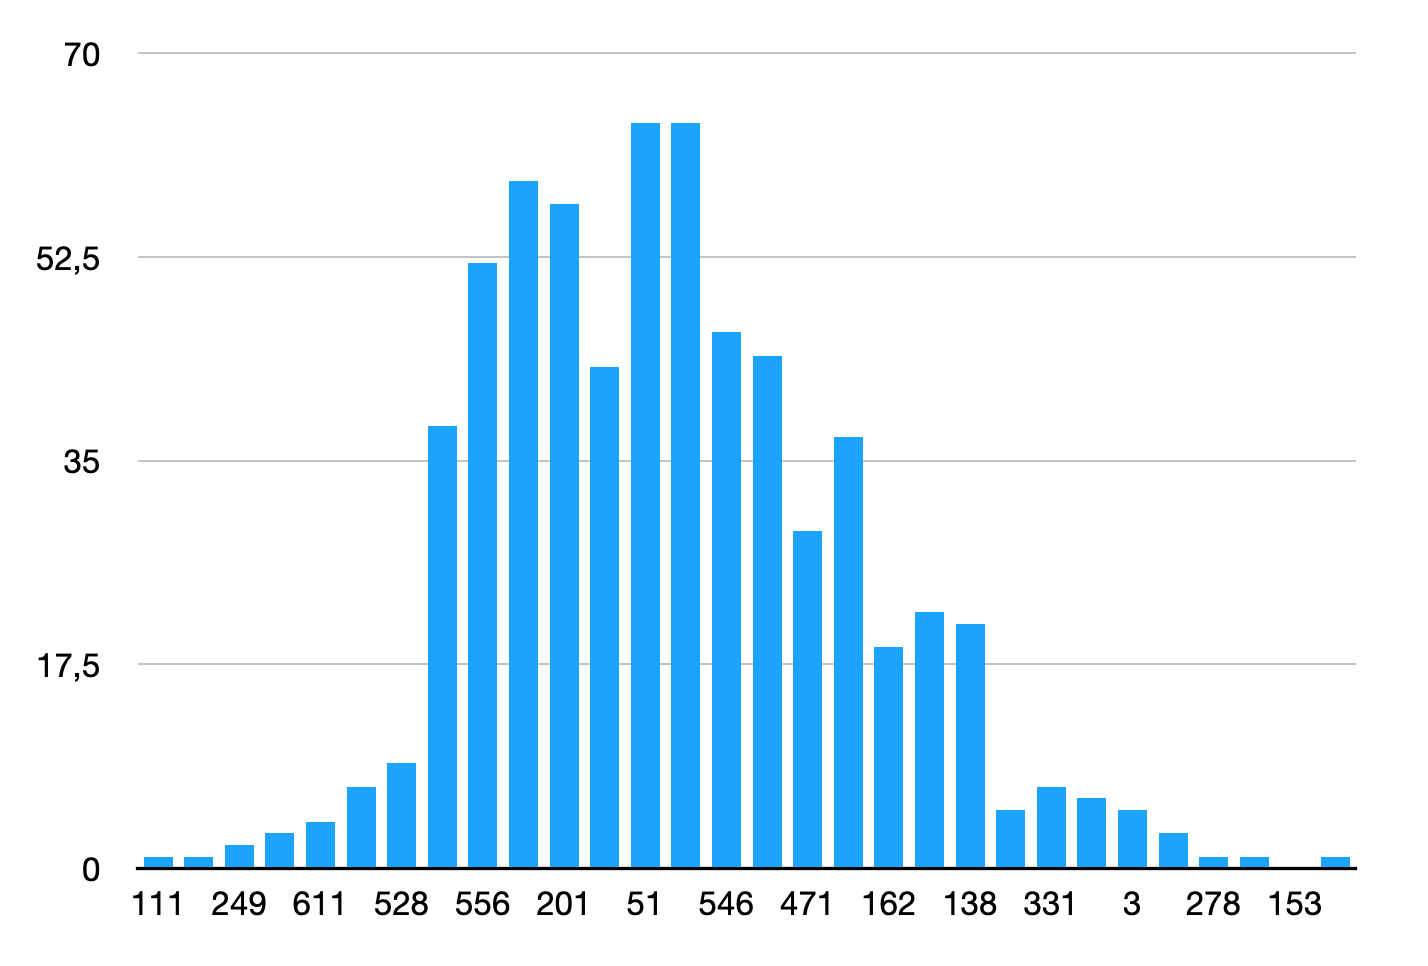
\includegraphics[width=6cm,height=4cm]{Overall por Periodos.png}
    \caption{Overall por Períodos}
    \label{fig:my_label}
\end{figure}
Com isso fica visível que é um um exemplo que se enquadra em distribuição padrão. E assim vemos que é relativamente um bom método para qualificar os times. Para termos noção esses são os cinco maiores e menores em questão de Overall:
\begin{figure}[H]
\centering
\subfigure[Top 5 Maiores Overall\label\{]{
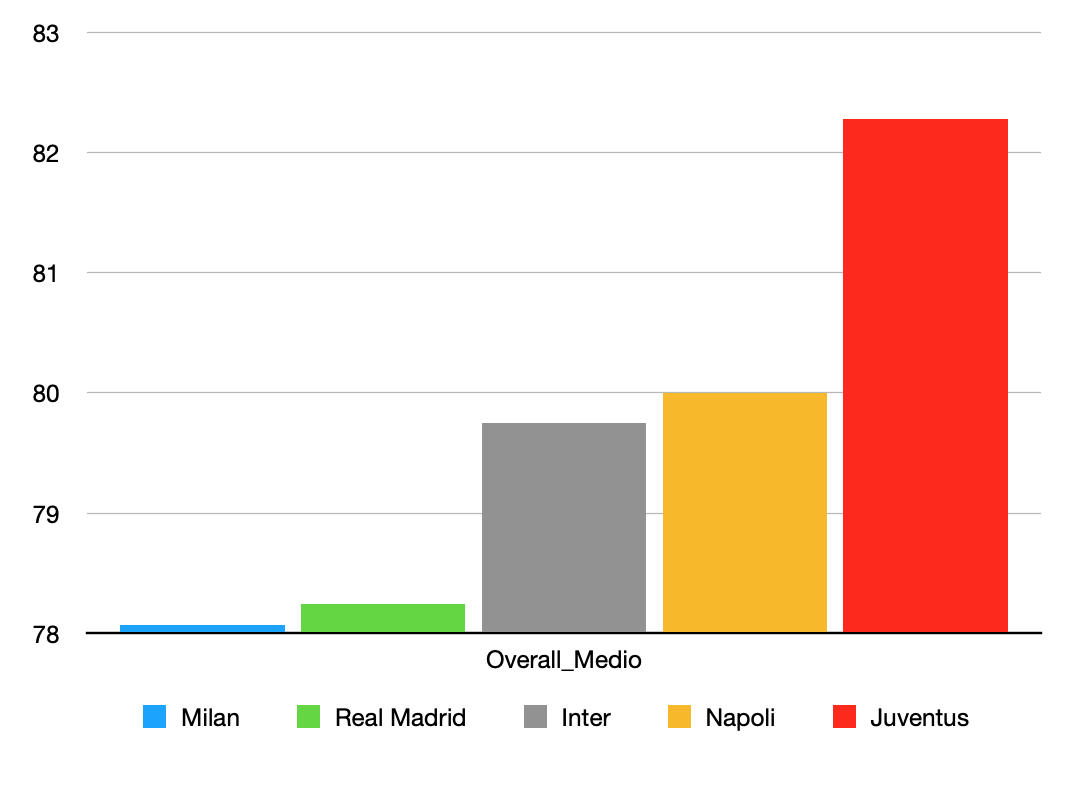
\includegraphics[width=5cm,height=3cm]{Top 5 Maiores Overalls.png}}
\subfigure[Top 5 Menores Overall\label{}]{
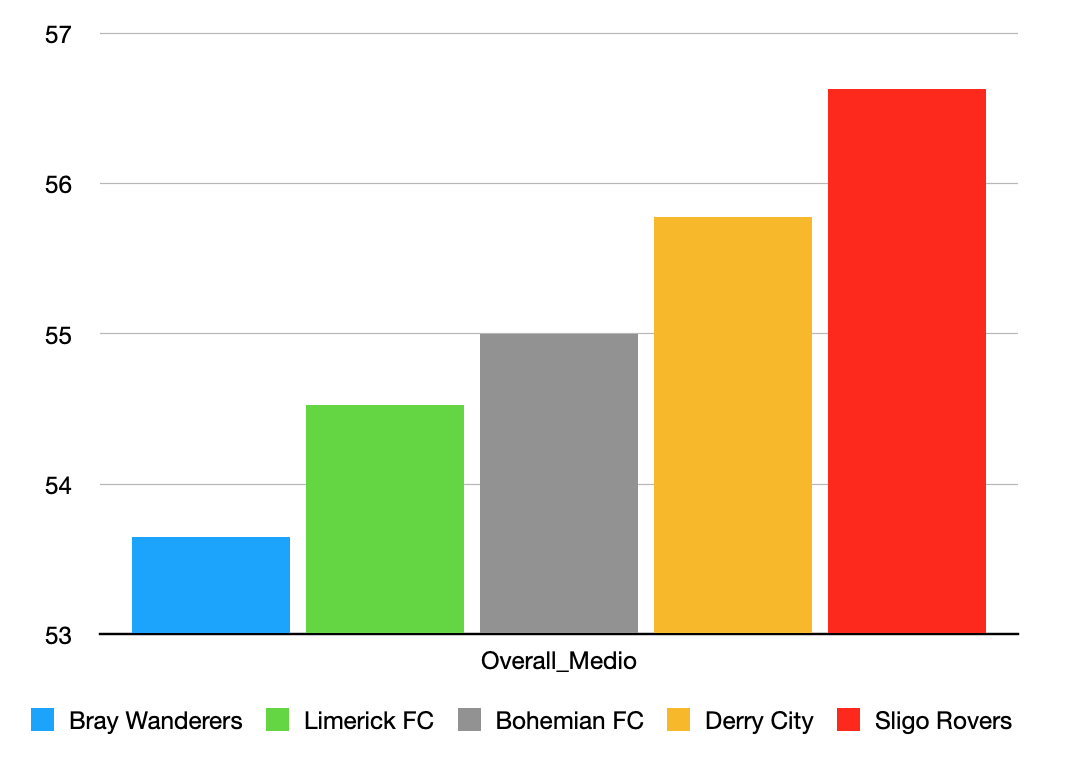
\includegraphics[width=5cm,height=3cm]{Top 5 Menores Overall.png}}
\end{figure} \\

\textbf{3.} Distribuição de Idade Média por Times
\begin{figure}[H]
    \centering
    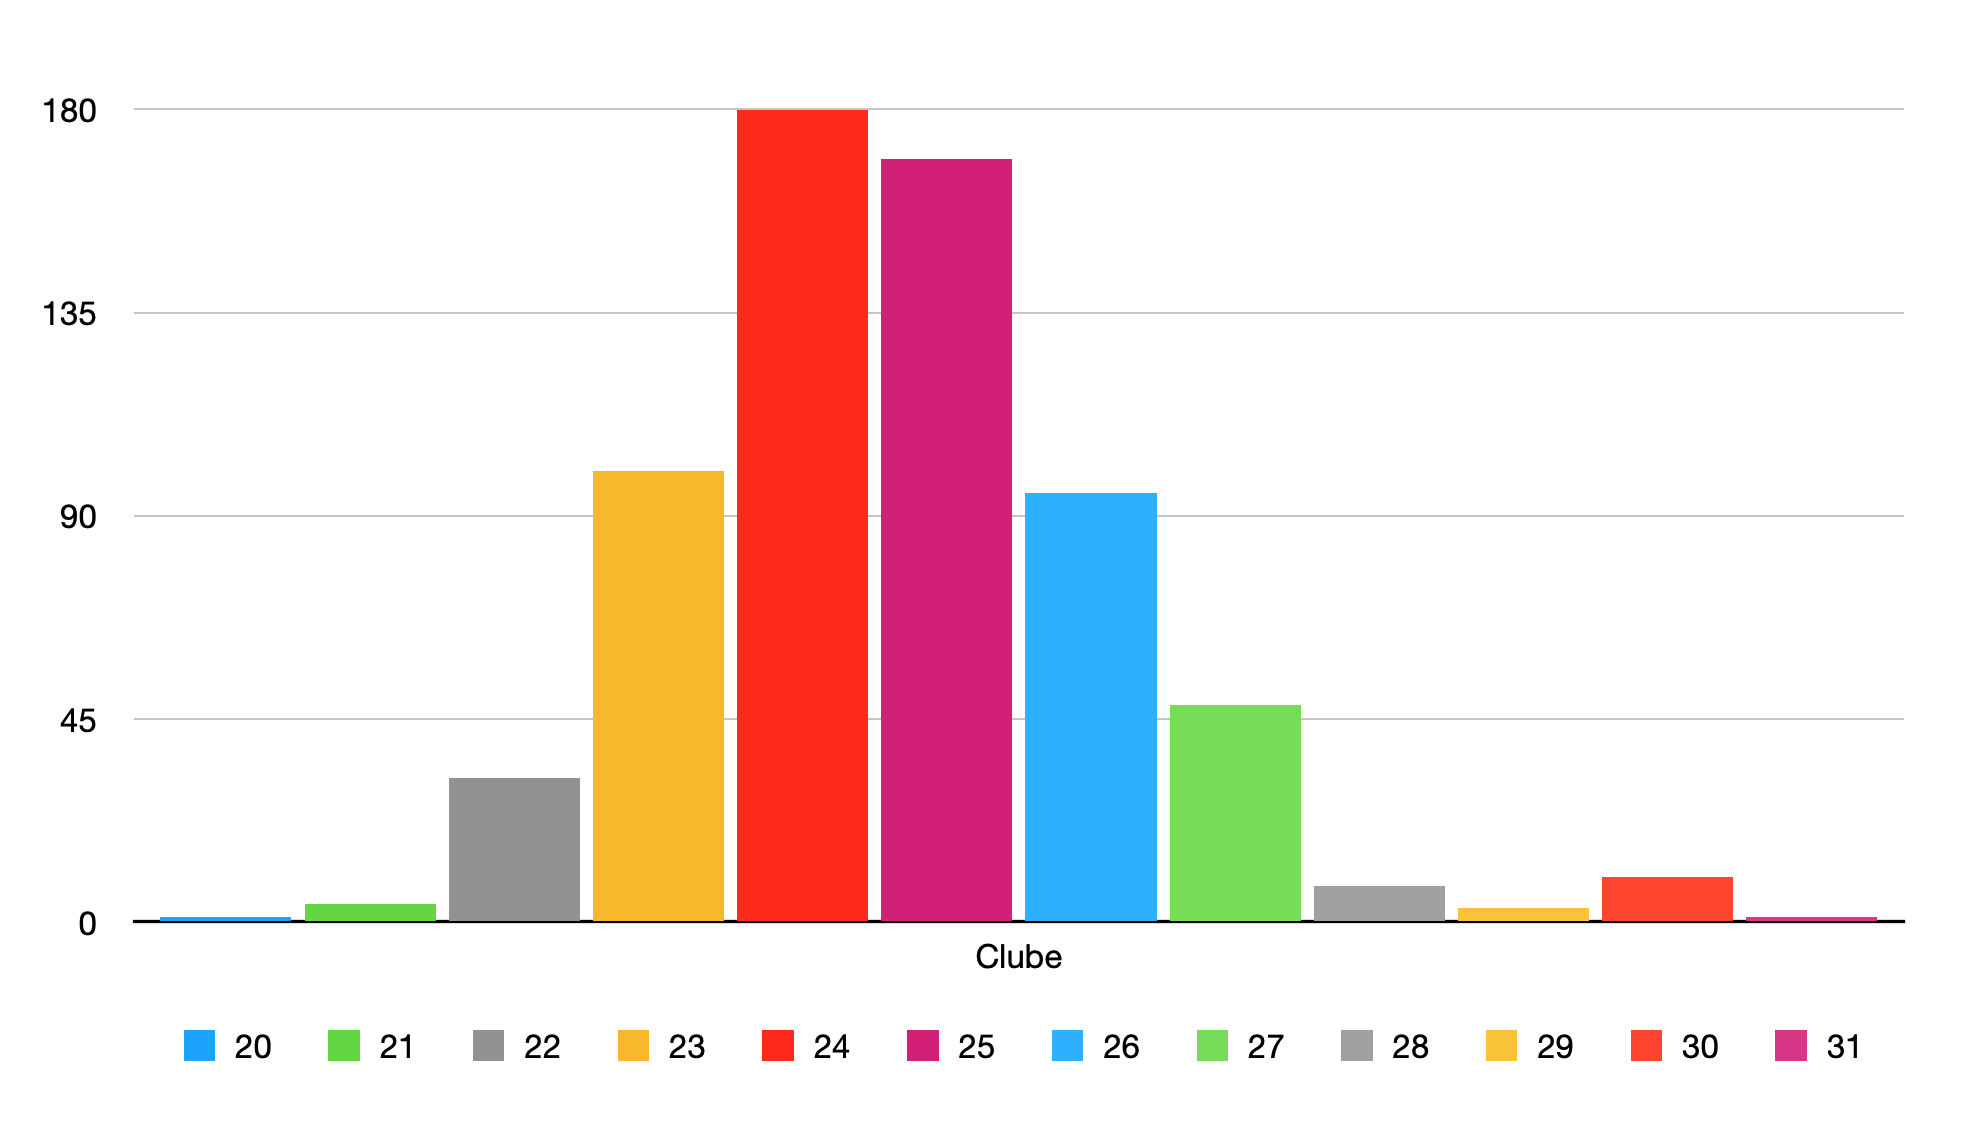
\includegraphics[width=6cm,height=4cm]{Distribuição de Idade Média dos Times.png}
    \caption{Distribuição Idade Média dos Times}
    \label{fig:my_label}
\end{figure}
Com isso podemos ver que a tendencia no futebol é os jogadores terem uma média de $25$ anos, que normalmente é a idade que eles estão com um melhor condicionamento físico. Novamente vemos a distribuição normal, o que faz muito sentido, pois raros são os jogadores muito novos que jogam nos times, e pouquíssimos os mais velhos. Pelo database existem $8108$ jogadores acima da idade média.\\

\textbf{4.} Distribuição de Destros e Canhotos por Posição
\begin{figure}[H]
    \centering
    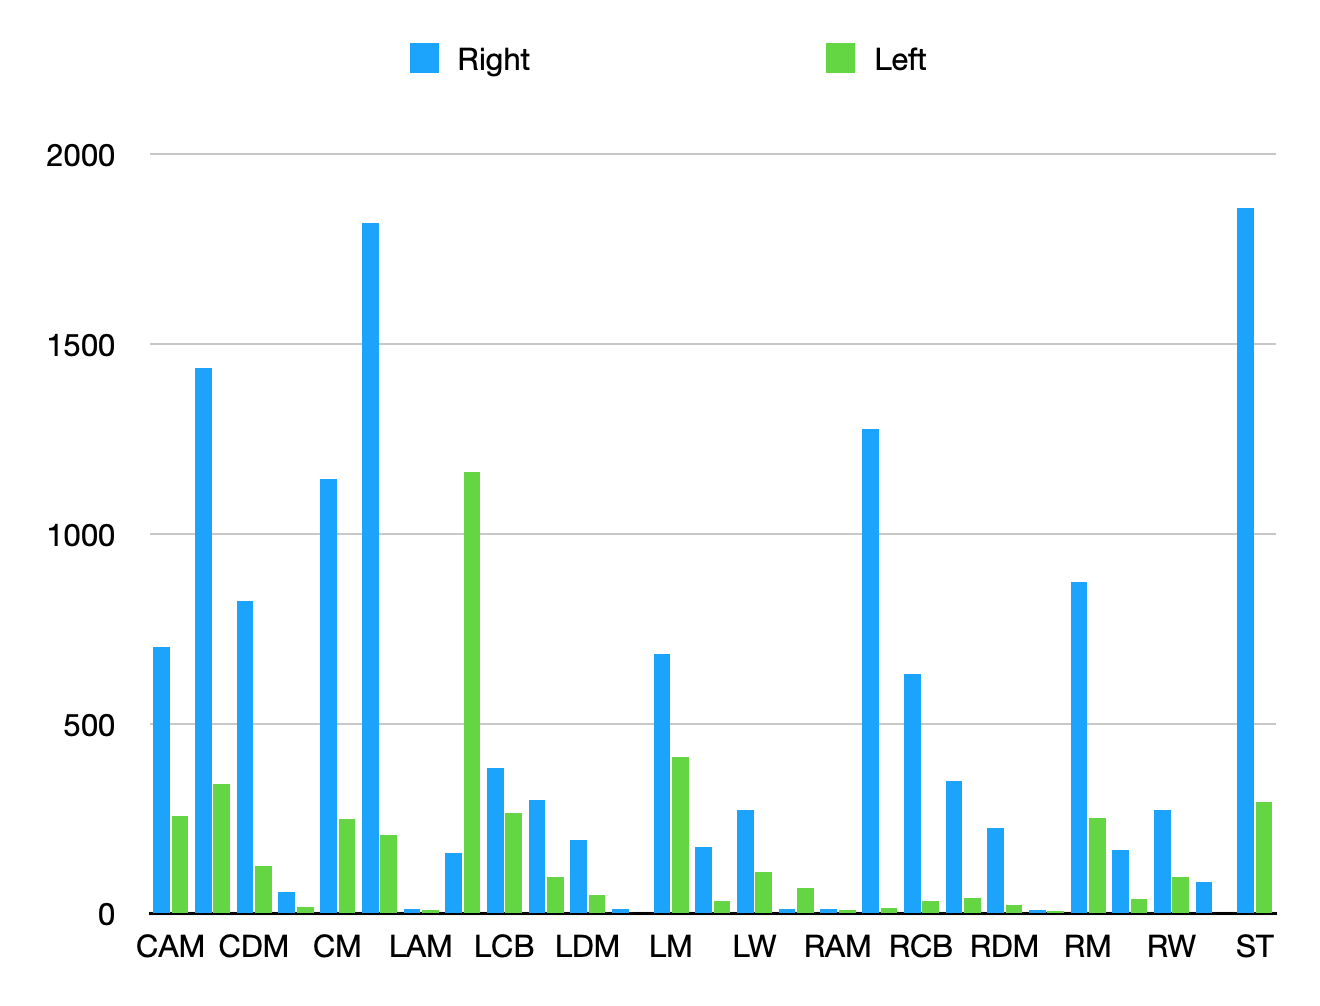
\includegraphics[width=6cm,height=4cm]{Relação Destro e Canhoto por Posição.png}
    \caption{Relação Destro e Canhoto por Posição}
    \label{fig:my_label}
\end{figure}
Atualmente no mundo, cerca de $10\%$ das pessoas são canhotas, havendo uma predominância de destro. No futebol é o mesmo, mas duas das posições chamam a atenção, que são a \textit{LB} e\textit{ LWB}, posições referentes a Defesa da Esquerda. Logo faz sentido ter essa discrepância, mas então porque o ataque pela esquerda também não tem essa diferença? Não a uma explicação concreta, muito provavelmente por existir mais destros mesmos, porém vale ressaltar que dos $22\% $ dos jogadores de alto nível são canhotos, uma diferença bem grande para os $10\%$.

\newpage
\textbf{4.} Relação entre Overall e Potencial
\begin{figure}[H]
    \centering
    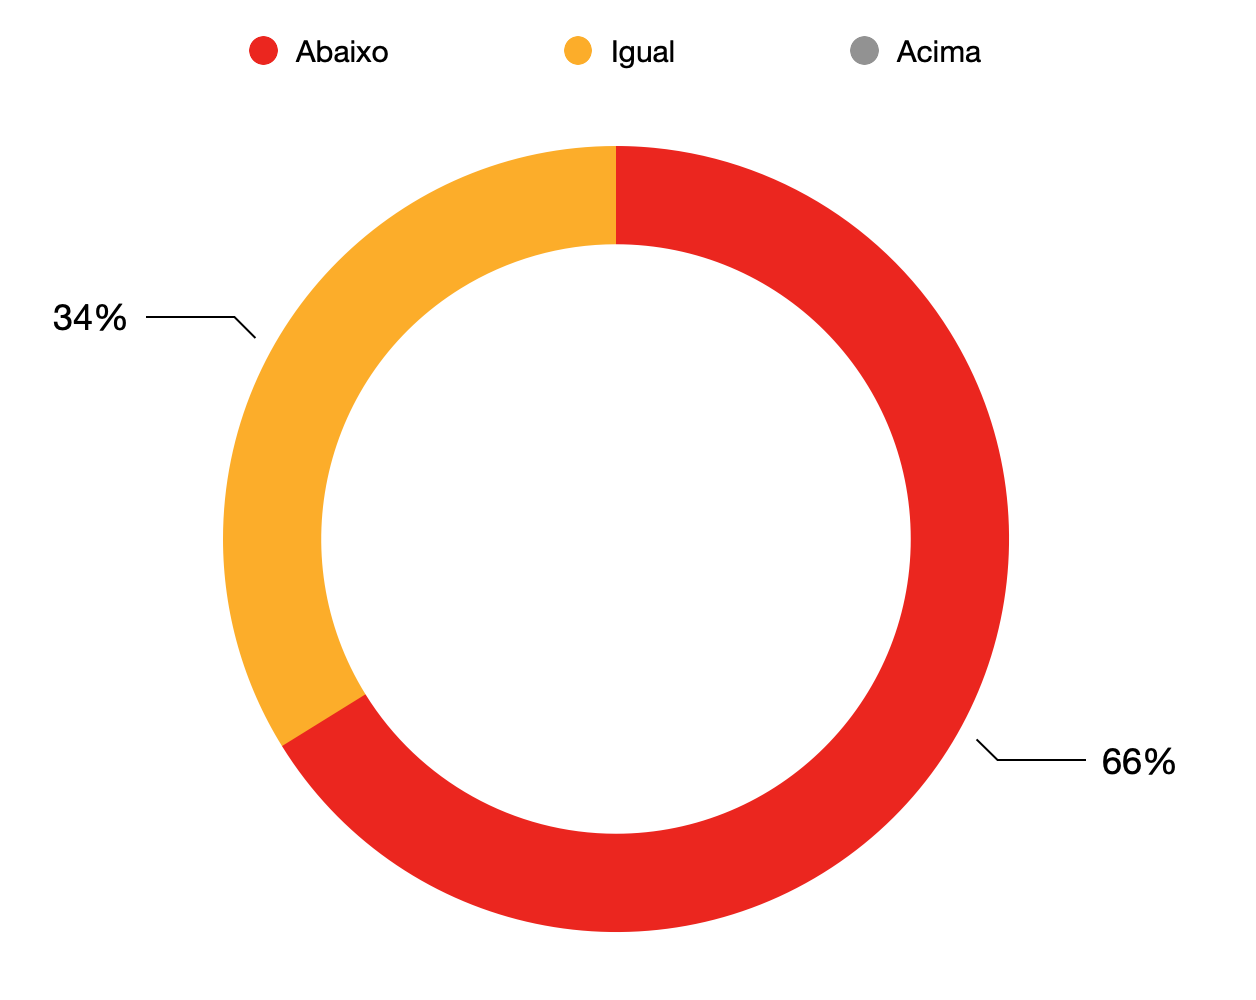
\includegraphics[width=5cm,height=4cm]{Relação entre Overall e Potencial.png}
    \caption{ Relação entre Overall e Potencial}
    \label{fig:my_label}
\end{figure}

Notasse que dois terços dos jogadores possuem um Overall menor que o Potencial e quando vemos quantos são iguais cai para um terço, mostrando que esses jogadores joga aproveitando o potencial máximo dele. Nenhum tem Overall maior que o Potencial,  o que é esperado, pois nenhum joga mais do que o máximo esperado dele, porque se jogasse, aquele não seria o seu máximo.

\section{GitHub}
Link do GitHub:
(\textbf{https://github.com/BrenoEmap/A2_ LP})\footnote[1]{\textcolor{blue}{\url{https://github.com/BrenoEmap/A2_LP}}}





\end{document}
